\documentclass[aspectratio=169, lualatex, handout]{beamer}
\makeatletter\def\input@path{{theme/}}\makeatother\usetheme{cipher}

\title{Applied Cryptography - 2.6: Post-Quantum Cryptography}
\author{Nadim Kobeissi}
\subject{An introduction to post-quantum cryptography covering the quantum threat to current cryptographic systems and new quantum-resistant algorithms like Learning with Errors (LWE).}
\keywords{post-quantum cryptography, quantum computing, Shor's algorithm, Grover's algorithm, Learning with Errors, LWE, lattice-based cryptography, CRYSTALS-Kyber, key encapsulation, NIST PQC}
\institute{American University of Beirut}
\instituteimage{images/aub-white.png}
\date{\today}
\coversubtitle{CMPS 297AD/396AI\\Fall 2025}
\coverpartname{Part 2: Real-World Cryptography}
\covertopicname{2.6: Post-Quantum Cryptography}
\coverwebsite{https://appliedcryptography.page}

\begin{document}
\begin{frame}[plain]
	\titlepage
\end{frame}

\section{Why Go Post-Quantum?}

\begin{frame}{The quantum threat}
	\begin{itemize}
		\item \textbf{Quantum computers} are fundamentally different from classical computers
		\item They exploit quantum mechanical phenomena: superposition and entanglement
		\item Can solve certain problems exponentially faster than classical computers
		\item \textbf{Critical insight}: Many cryptographic algorithms rely on problems that quantum computers can solve efficiently
	\end{itemize}
\end{frame}

\begin{frame}{How quantum computers work}
	\begin{itemize}
		\item \textbf{Classical bits}: Can be either 0 or 1
		\item \textbf{Quantum bits (qubits)}: Can be in \textit{superposition} of 0 and 1 simultaneously
		\item \textbf{Superposition}: A qubit can represent both states at once
		      \begin{itemize}
			      \item $n$ classical bits: Store one of $2^n$ possible values
			      \item $n$ qubits: Can represent all $2^n$ values simultaneously
		      \end{itemize}
		\item \textbf{Entanglement}: Qubits can be correlated in ways impossible classically
		      \begin{itemize}
			      \item Measuring one qubit instantly affects others
			      \item Enables parallel computation across exponentially many states
		      \end{itemize}
		\item \textbf{Quantum parallelism}: Process all possibilities at once, extract answer through interference
	\end{itemize}
\end{frame}

\begin{frame}{Building quantum computers: the engineering challenge}
	\begin{itemize}
		\item \textbf{Multiple approaches being pursued}:
		      \begin{itemize}
			      \item Superconducting circuits (IBM, Google)
			      \item Trapped ions (IonQ, Honeywell)
			      \item Topological qubits (Microsoft)
			      \item Photonic qubits (Xanadu, PsiQuantum)
			      \item Neutral atoms (QuEra, Pasqal)
		      \end{itemize}
		\item \textbf{Common requirement}: Maintain quantum coherence
		      \begin{itemize}
			      \item Qubits must remain in superposition
			      \item Any interaction with environment causes \textit{decoherence}
			      \item Current coherence times: microseconds to milliseconds
		      \end{itemize}
	\end{itemize}
\end{frame}

\begin{frame}{Physical challenges: Why qubits are so difficult}
	\begin{itemize}
		\item \textbf{Size requirements}: Qubits are difficult to physically manipulate
		      \begin{itemize}
			      \item Individual photons, electrons, or atomic nuclei
			      \item Some approaches (superconducting) have larger qubits
			      \item Impossible to manipulate with conventional tools
			      \item Require laser beams or electromagnetic fields for control
		      \end{itemize}
		\item \textbf{Temperature requirements}: Near absolute zero (-273\degree\ C)
		      \begin{itemize}
			      \item For some quantum systems, tiny amounts of heat destroy quantum states
			      \item Requires dilution refrigerators costing millions
			      \item More cooling power needed as system scales
		      \end{itemize}
		\item \textbf{Isolation from environment}:
		      \begin{itemize}
			      \item Magnetic fields, vibrations, cosmic rays all cause errors
			      \item Need multiple layers of shielding
			      \item Even observation destroys quantum states!
		      \end{itemize}
	\end{itemize}
\end{frame}

\begin{frame}{The coherence problem: Racing against time}
	\begin{itemize}
		\item \textbf{Coherence time}: How long qubits maintain their quantum state
		      \begin{itemize}
			      \item Current record: A few seconds at best
			      \item Most systems: Microseconds to milliseconds
			      \item Breaking crypto needs: Days to weeks of computation
		      \end{itemize}
		\item \textbf{Error rates}: Quantum operations are inherently noisy
		      \begin{itemize}
			      \item Classical computers: 1 error per $10^{17}$ operations
			      \item Current quantum computers: 1 error per $10^{3}$ operations
			      \item Need massive improvement to be useful
		      \end{itemize}
		\item \textbf{Quantum error correction}:
		      \begin{itemize}
			      \item Can't copy quantum states (no-cloning theorem)
			      \item Need 100-1000 physical qubits to make 1 logical qubit
			      \item Turns ``millions of qubits'' into ``billions of physical qubits''
		      \end{itemize}
	\end{itemize}
\end{frame}

\begin{frame}{What makes current cryptography vulnerable?}
	\begin{itemize}
		\item \textbf{RSA}: Based on factoring large integers
		\item \textbf{Diffie-Hellman}: Based on discrete logarithm problem
		\item \textbf{Elliptic Curve Cryptography}: Also based on discrete logarithm problem
		\item These are \textit{hard} for classical computers but \textit{easy} for quantum computers
		\item \textbf{Shor's algorithm} (1994): Polynomial-time quantum algorithm for factoring and discrete log
	\end{itemize}
\end{frame}

\begin{frame}{Grover's algorithm: summary}
	\begin{itemize}
		\item \textbf{Grover's algorithm}: Quantum algorithm for searching unsorted databases
		\item \textbf{Classical search}: $\mathcal{O}(2^n)$ time to search $2^n$ items
		\item \textbf{Quantum search}: $O(2^{n/2})$ time with Grover's algorithm
		\item \textbf{Formal claim}: Given $F: \{0,1\}^n \rightarrow \{0,1\}$, Grover's algorithm makes $O(2^{n/2})$ quantum evaluations of $F$ and outputs $X \in \{0,1\}^n$ such that $F(X) = 1$, if such $X$ exists
		\item \textbf{Intuition}: Finding needles in haystacks
		      \begin{itemize}
			      \item Haystack: $\{0,1\}^n$ (all possible inputs)
			      \item Needle: Special input $X$ where $F(X) = 1$
		      \end{itemize}
	\end{itemize}
\end{frame}

\begin{frame}{Grover's algorithm: attacking symmetric cryptography}
	\begin{columns}[c]
		\begin{column}{1\textwidth}
			\begin{itemize}
				\item \textbf{Attack setup}: Obtain known plaintext-ciphertext pairs
				      \begin{itemize}
					      \item $C_1 = \text{Enc}(K, M_1)$, $C_2 = \text{Enc}(K, M_2)$, ..., $C_m = \text{Enc}(K, M_m)$
				      \end{itemize}
				\item \textbf{Define search function}:
				      \begin{align*}
					      F(K) = \begin{cases}
						             1 & \text{if } \text{Dec}(K, C_i) = M_i \text{ for all } i \\
						             0 & \text{otherwise}
					             \end{cases}
				      \end{align*}
				\item \textbf{Result}: Grover finds the correct key in $O(2^{\lambda/2})$ time\footnote{Note: Grover's algorithm is inherently sequential (cannot be parallelized efficiently)}
				\item \textbf{Defense}: Double the key size\footnote{Cryptographers argue about this recommendation in different points, some thinking it's too simplistic, others thinking that with hash functions, you may not need to go from SHA-256 to SHA-512 with SHA-384 being enough, etc.}
				      \begin{itemize}
					      \item AES-128 $\rightarrow$ AES-256 (to maintain 128-bit security)
					      \item SHA-256 $\rightarrow$ SHA-512 (for collision resistance)
				      \end{itemize}
			\end{itemize}
		\end{column}
	\end{columns}
\end{frame}

\begin{frame}{Shor's algorithm: summary}
	\begin{itemize}
		\item In 1994, Peter Shor demonstrated that quantum computers could break most asymmetric-key cryptography in polynomial time
		\item \textbf{Claim}: There are quantum algorithms for the following tasks, whose running time is polynomial in $k$:
		      \begin{itemize}
			      \item Factoring $k$-bit numbers
			      \item Solving the discrete logarithm problem in any cyclic group of order $< 2^k$, even groups based on elliptic curves
		      \end{itemize}
		\item Both algorithms use a common approach called \textit{Shor's algorithm}
		\item \textbf{Implication}: All public-key cryptography based on factoring (RSA) or discrete logarithm (Diffie-Hellman, El Gamal, Schnorr) can be broken by quantum computers
	\end{itemize}
\end{frame}

\begin{frame}{Shor's algorithm: impact}
	\begin{columns}[c]
		\begin{column}{0.5\textwidth}
			\begin{itemize}
				\item Classical factoring: Best known algorithm takes exponential time
				\item Quantum factoring with Shor's: Takes polynomial time
				\item Example: Factoring a 2048-bit RSA key
				      \begin{itemize}
					      \item Classical: Billions of years
					      \item Quantum: Hours to days (with a large enough quantum computer)
				      \end{itemize}
				\item \textbf{Impact}: Complete break of RSA, ECC, and DH key exchange
			\end{itemize}
		\end{column}
		\begin{column}{0.5\textwidth}
			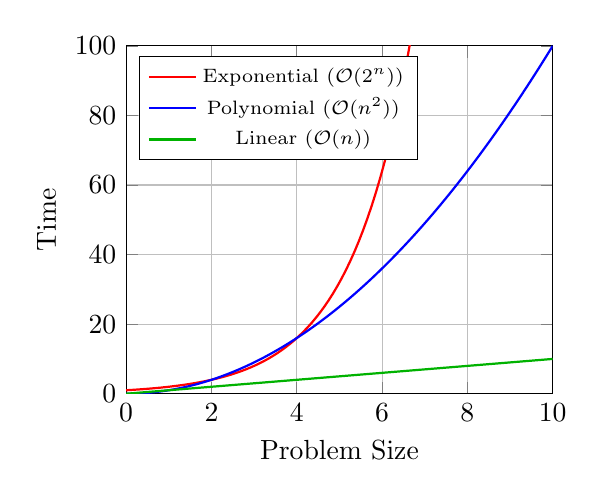
\begin{tikzpicture}[scale=1]
				\begin{axis}[
						xlabel={Problem Size},
						ylabel={Time},
						xmin=0, xmax=10,
						ymin=0, ymax=100,
						legend pos=north west,
						legend style={font=\scriptsize, align=left},
						grid=major,
						width=7cm,
						height=6cm,
					]
					\addplot[red, thick, domain=0:10, samples=100] {2^x};
					\addlegendentry{Exponential ($\mathcal{O}(2^n)$)}
					\addplot[blue, thick, domain=0:10, samples=100] {x^2};
					\addlegendentry{Polynomial ($\mathcal{O}(n^2)$)}
					\addplot[green!70!black, thick, domain=0:10] {x};
					\addlegendentry{Linear ($\mathcal{O}(n)$)}
				\end{axis}
			\end{tikzpicture}
		\end{column}
	\end{columns}
\end{frame}

\begin{frame}{Not all cryptography is equally vulnerable}
	\begin{columns}[c]
		\begin{column}{1\textwidth}
			\begin{itemize}
				\item \textbf{Asymmetric cryptography}: Severely impacted by quantum computers
				      \begin{itemize}
					      \item RSA, ECC, DH $\rightarrow$ Completely broken by Shor's algorithm
				      \end{itemize}
				\item \textbf{Symmetric cryptography}: Less impacted
				      \begin{itemize}
					      \item AES, SHA-256 $\rightarrow$ Weakened but not broken
					      \item Grover's algorithm: Provides quadratic speedup
					      \item Solution: Double the key size (AES-128 $\rightarrow$ AES-256)\footnote{Cryptographers argue about this recommendation in different points, some thinking it's too simplistic, others thinking that with hash functions, you may not need to go from SHA-256 to SHA-512 with SHA-384 being enough, etc.}
				      \end{itemize}
				\item \textbf{Hash functions}: Similar to symmetric crypto
				      \begin{itemize}
					      \item Need larger output sizes to maintain security
				      \end{itemize}
			\end{itemize}
		\end{column}
	\end{columns}
\end{frame}

\begin{frame}{Timeline: when will quantum computing arrive?}
	\begin{itemize}
		\item \textbf{Current state}: Small quantum computers exist (100s of qubits)
		\item \textbf{Required for cryptanalysis}: Millions of error-corrected qubits
		\item \textbf{Expert predictions}: 10-30 years until cryptographically relevant quantum computers (depending on who you ask)
		\item \textbf{But consider}:
		      \begin{itemize}
			      \item Technological breakthroughs could accelerate timeline
			      \item Nation-states investing billions in quantum research
			      \item Progress has been faster than expected in recent years
		      \end{itemize}
	\end{itemize}
\end{frame}

\begin{frame}{Timeline: when will quantum computing arrive?}
	\bigimagewithcaption{quantum-threat.png}{Source: Michele Mosca and Marco Piani, Quantum Threat Timeline Report, Global Risk Institute, 2024.}
\end{frame}

\begin{frame}{Timeline: according to Sam Jaques}
	\bigimagewithcaption{quantum-timeline.png}{Source: Sam Jaques}
\end{frame}

\begin{frame}{Reality check: Current quantum factorization records}
	\begin{itemize}
		\item \textbf{2001}: IBM factored $15 = 3 \times 5$ using Shor's algorithm
		\item \textbf{2012}: Factored $21 = 3 \times 7$
		\item \textbf{2019}: Attempted to factor $35 = 5 \times 7$
		\item \textbf{In 24 years}: Progress from 15 to 21
		\item \textbf{For context}: A 1981 VIC-20 home computer can factor these numbers instantly
		\item These aren't even true applications of Shor's algorithm - they use ``compiled'' versions with prior knowledge of the answer
	\end{itemize}
\end{frame}

\begin{frame}{Alternative ``quantum'' factorization methods}
	\begin{columns}[c]
		\begin{column}{1\textwidth}
			\begin{itemize}
				\item Recent paper\footnote{\url{https://appliedcryptography.page/paper/\#quantum-dog}} demonstrates matching all quantum factorization records using:
				      \begin{itemize}
					      \item \textbf{VIC-20}: 8-bit computer from 1981 (538 bytes of code)
					      \item \textbf{Abacus}: Ancient counting device
					      \item \textbf{Dog}: Trained to bark 3 times (factors 15 and 21)
				      \end{itemize}
				\item All methods successfully factor every number claimed by quantum computers
				\item The VIC-20 can factor the RSA-2048 ``quantum'' examples in 16.5 seconds
				\item \textbf{Conclusion}: Current quantum computers offer no practical advantage
			\end{itemize}
		\end{column}
	\end{columns}
\end{frame}

\begin{frame}{The sleight-of-hand problem}
	\begin{itemize}
		\item Most quantum factorization claims use specially constructed ``sleight-of-hand'' numbers
		\item \textbf{Example}: RSA-2048 ``factorization'' claims
		      \begin{itemize}
			      \item Factors chosen to differ by only 2 or 6
			      \item Real RSA keys require factors to differ by >100 bits
			      \item Can be factored with simple square root calculation
		      \end{itemize}
		\item \textbf{Common tricks}:
		      \begin{itemize}
			      \item Numbers with special binary patterns (mostly zeros)
			      \item Preprocessing on classical computers
			      \item ``Compiled'' algorithms that know the answer in advance
		      \end{itemize}
	\end{itemize}
\end{frame}

\begin{frame}{The gap between hype and reality}
	\begin{itemize}
		\item \textbf{Claimed}: ``RSA-2048 factored by quantum computer''
		\item \textbf{Reality}: Used specially constructed weak keys, solvable on 1980s hardware
		\item \textbf{Estimated timeline}: 10-30 years to cryptographically relevant quantum computers
		\item \textbf{Historical note}: Similar timeline estimates have been made for decades
		\item \textbf{Critical question}: Should we redesign all cryptography based on devices that can't outperform a dog?
	\end{itemize}
\end{frame}

\begin{frame}{Store now, decrypt later}
	\begin{itemize}
		\item \textbf{The problem}: Adversaries can store encrypted data today
		\item Wait for quantum computers to become available
		\item Decrypt all previously recorded communications
		\item \textbf{Implications}:
		      \begin{itemize}
			      \item Data encrypted today may be decrypted in 10-20 years
			      \item Long-term secrets are already at risk
			      \item Medical records, government communications, trade secrets
		      \end{itemize}
		\item \textbf{This attack is happening NOW}
		\item This is why some argue that we can't just not do anything because quantum computers seem impractical \textit{today}
	\end{itemize}
\end{frame}

\begin{frame}{Why transition now?}
	\begin{itemize}
		\item \textbf{Migration takes time}: Historical crypto transitions took 10-20 years
		      \begin{itemize}
			      \item Recall the transition away from RC4, seen earlier in the course!
		      \end{itemize}
		\item \textbf{Complex systems}: Need to update protocols, libraries, hardware
		\item \textbf{Backward compatibility}: Must support both old and new systems
		\item \textbf{Unknown vulnerabilities}: New algorithms need time for analysis
		\item \textbf{Compliance and standards}: Regulations take years to update
		\item \textbf{Bottom line}: If we wait until quantum computers exist, it's too late
	\end{itemize}
\end{frame}

\section{Going Post-Quantum}

\begin{frame}{Post-quantum cryptography: the solution}
	\begin{itemize}
		\item \textbf{Definition}: Cryptographic algorithms that are secure against both classical and quantum computers
		\item Based on mathematical problems believed to be hard even for quantum computers:
		      \begin{itemize}
			      \item Lattice-based problems
			      \item Code-based problems
			      \item Hash-based signatures
			      \item Multivariate polynomial equations
			      \item Isogeny-based problems
		      \end{itemize}
		\item \textbf{Goal}: Deploy these before quantum computers arrive
	\end{itemize}
\end{frame}

\begin{frame}{The NIST Post-Quantum Cryptography Competition}
	\begin{itemize}
		\item Started in 2016 to standardize post-quantum algorithms
		\item 69 initial submissions $\rightarrow$ Multiple rounds of analysis
		\item \textbf{2022}: First algorithms standardized
		      \begin{itemize}
			      \item \textbf{CRYSTALS-Kyber}: Key encapsulation (KEM)
			      \item \textbf{CRYSTALS-Dilithium}: Digital signatures
			      \item \textbf{FALCON}: Digital signatures
			      \item \textbf{SPHINCS+}: Hash-based signatures
		      \end{itemize}
		\item Global effort: Cryptographers worldwide analyzing security
	\end{itemize}
\end{frame}

\begin{frame}{Real-world impact: who needs to care?}
	\begin{itemize}
		\item \textbf{Financial institutions}: Protecting transactions and customer data
		\item \textbf{Healthcare}: Medical records must remain private for decades
		\item \textbf{Government}: National security and citizen privacy
		\item \textbf{Technology companies}: Secure communications and data storage
		\item \textbf{Critical infrastructure}: Power grids, water systems, transportation
		\item \textbf{Everyone}: Personal communications, passwords, private data
	\end{itemize}
\end{frame}

\begin{frame}{Starting at the left}
	\bigimagewithcaption{fischer.png}{Fischer et al., The Challenges of Bringing Cryptography from Research Papers to Products: Results from an Interview Study with Experts, USENIX Security 2024}
\end{frame}

\subsection{Learning with Errors}

\begin{frame}{The Learning with Errors (LWE) Problem}
	\begin{itemize}
		\item \textbf{Key insight}: Some mathematical problems remain hard even for quantum computers
		\item \textbf{LWE}: Based on solving noisy systems of linear equations
		\item \textbf{Security foundation}: The difficulty of distinguishing random noise from structured noise
		\item Forms the basis for many post-quantum cryptographic schemes
		\item First, let's see why regular linear equations are easy\ldots
	\end{itemize}
\end{frame}

\begin{frame}{Solving linear equations: the easy case}
	\begin{itemize}
		\item Consider solving for unknowns $s_1, s_2, s_3, s_4, s_5$ in:
	\end{itemize}
	\begin{align*}
		3 & = s_1 + 2s_2 - 2s_3 + 6s_5         \\
		1 & = 4s_1 + 3s_2 - 4s_3 - 3s_4 + 6s_5 \\
		4 & = -s_1 - s_2 + 4s_3 + 3s_4 - 3s_5  \\
		1 & = s_1 - s_2 + 2s_3 + 3s_4 + s_5    \\
		5 & = 4s_1 + 5s_2 + 5s_3 + 3s_4 + s_5
	\end{align*}
	\begin{itemize}
		\item We know an efficient algorithm for this
	\end{itemize}
\end{frame}

\begin{frame}{Matrix form of linear equations}
	The system can be written as:
	\begin{columns}[c]
		\begin{column}{0.5\textwidth}
			\begin{align*}
				3 & = s_1 + 2s_2 - 2s_3 + 6s_5         \\
				1 & = 4s_1 + 3s_2 - 4s_3 - 3s_4 + 6s_5 \\
				4 & = -s_1 - s_2 + 4s_3 + 3s_4 - 3s_5  \\
				1 & = s_1 - s_2 + 2s_3 + 3s_4 + s_5    \\
				5 & = 4s_1 + 5s_2 + 5s_3 + 3s_4 + s_5
			\end{align*}
		\end{column}
		\begin{column}{0.5\textwidth}
			\[
				\begin{bmatrix}
					3 \\ 1 \\ 4 \\ 1 \\ 5
				\end{bmatrix}
				=
				\begin{bmatrix}
					1  & 2  & -2 & 0  & 6  \\
					4  & 3  & -4 & -3 & 6  \\
					-1 & -1 & 4  & 3  & -3 \\
					1  & -1 & 2  & 3  & 1  \\
					4  & 5  & 5  & 3  & 1
				\end{bmatrix}
				\begin{bmatrix}
					s_1 \\ s_2 \\ s_3 \\ s_4 \\ s_5
				\end{bmatrix}
			\]
		\end{column}
	\end{columns}
	\vspace{5mm}
	\begin{itemize}
		\item Solution: Invert the matrix and multiply
		\item Polynomial time algorithm exists
		\item Adding more constraints (rows) doesn't make it harder
	\end{itemize}
\end{frame}

\begin{frame}{What is Gaussian elimination?}
	\begin{itemize}
		\item \textbf{Goal}: Solve systems of linear equations systematically
		\item \textbf{Basic idea}: Transform the system into a simpler form that's easy to solve
		\item \textbf{Method}: Use row operations to eliminate variables step by step
		\item \textbf{Notation}:
		      \begin{itemize}
			      \item $R_1$ = Row 1 (first equation)
			      \item $R_2$ = Row 2 (second equation)
			      \item $R_3$ = Row 3 (third equation), etc.
		      \end{itemize}
		\item We'll work with an \textbf{augmented matrix}: the coefficient matrix with the constants column attached
	\end{itemize}
\end{frame}

\begin{frame}{Step 1: Set up the augmented matrix}
	\begin{columns}[c]
		\begin{column}{0.5\textwidth}
			Start with the system:
			\begin{align*}
				3 & = s_1 + 2s_2 - 2s_3 + 6s_5         \\
				1 & = 4s_1 + 3s_2 - 4s_3 - 3s_4 + 6s_5 \\
				4 & = -s_1 - s_2 + 4s_3 + 3s_4 - 3s_5  \\
				1 & = s_1 - s_2 + 2s_3 + 3s_4 + s_5    \\
				5 & = 4s_1 + 5s_2 + 5s_3 + 3s_4 + s_5
			\end{align*}
		\end{column}
		\begin{column}{0.5\textwidth}
			Create augmented matrix $[A|b]$:
			\[
				\left[\begin{array}{ccccc|c}
						1  & 2  & -2 & 0  & 6  & 3 \\
						4  & 3  & -4 & -3 & 6  & 1 \\
						-1 & -1 & 4  & 3  & -3 & 4 \\
						1  & -1 & 2  & 3  & 1  & 1 \\
						4  & 5  & 5  & 3  & 1  & 5
					\end{array}\right]
			\]
			Each row represents one equation
		\end{column}
	\end{columns}
\end{frame}

\begin{frame}{What are row operations?}
	\textbf{Three allowed operations} (these don't change the solution):
	\begin{enumerate}
		\item \textbf{Multiply a row by a non-zero constant}
		      \begin{itemize}
			      \item Example: $R_1 \leftarrow 2R_1$ means ``multiply Row 1 by 2''
		      \end{itemize}
		\item \textbf{Add/subtract a multiple of one row to another}
		      \begin{itemize}
			      \item Example: $R_2 \leftarrow R_2 - 4R_1$ means ``subtract 4 times Row 1 from Row 2''
		      \end{itemize}
		\item \textbf{Swap two rows}
		      \begin{itemize}
			      \item Example: Swap $R_2$ and $R_3$
		      \end{itemize}
	\end{enumerate}
	\textbf{Our strategy}: Use these operations to create zeros below the diagonal
\end{frame}

\begin{frame}{Row operations: Concrete examples}
	\small
	\textbf{1. Multiply a row by a non-zero constant:}
	\[
		\left[\begin{array}{ccc|c}
				2 & 4 & 6 & 8 \\
				1 & 3 & 5 & 7 \\
				4 & 2 & 1 & 3
			\end{array}\right]
		\xrightarrow{R_1 \leftarrow \frac{1}{2}R_1}
		\left[\begin{array}{ccc|c}
				1 & 2 & 3 & 4 \\
				1 & 3 & 5 & 7 \\
				4 & 2 & 1 & 3
			\end{array}\right]
	\]

	\textbf{2. Add/subtract a multiple of one row to another:}
	\[
		\left[\begin{array}{ccc|c}
				1 & 2 & 3 & 4 \\
				1 & 3 & 5 & 7 \\
				4 & 2 & 1 & 3
			\end{array}\right]
		\xrightarrow{R_2 \leftarrow R_2 - R_1}
		\left[\begin{array}{ccc|c}
				1 & 2 & 3 & 4 \\
				0 & 1 & 2 & 3 \\
				4 & 2 & 1 & 3
			\end{array}\right]
	\]

	\textbf{3. Swap two rows:}
	\[
		\left[\begin{array}{ccc|c}
				1 & 2 & 3 & 4 \\
				0 & 1 & 2 & 3 \\
				4 & 2 & 1 & 3
			\end{array}\right]
		\xrightarrow{R_1 \leftrightarrow R_3}
		\left[\begin{array}{ccc|c}
				4 & 2 & 1 & 3 \\
				0 & 1 & 2 & 3 \\
				1 & 2 & 3 & 4
			\end{array}\right]
	\]
\end{frame}

\begin{frame}{Step 2a: Understanding the first elimination}
	\textbf{Goal}: Make all entries in column 1 (below row 1) equal to zero

	Current matrix:
	\[
		\left[\begin{array}{ccccc|c}
				\boxed{1}           & 2  & -2 & 0  & 6  & 3 \\
				\textcolor{red}{4}  & 3  & -4 & -3 & 6  & 1 \\
				\textcolor{red}{-1} & -1 & 4  & 3  & -3 & 4 \\
				\textcolor{red}{1}  & -1 & 2  & 3  & 1  & 1 \\
				\textcolor{red}{4}  & 5  & 5  & 3  & 1  & 5
			\end{array}\right]
	\]

	\begin{itemize}
		\item The boxed 1 is our \textbf{pivot} (the element we use to eliminate others)
		\item We want to turn the red numbers into zeros
	\end{itemize}
\end{frame}

\begin{frame}{Step 2b: Performing the eliminations}
	\begin{columns}[c]
		\begin{column}{0.6\textwidth}
			To eliminate the 4 in Row 2: subtract 4 times Row 1 from Row 2
			\begin{itemize}
				\item $R_2 \leftarrow R_2 - 4R_1$ means: $(4, 3, -4, -3, 6 | 1) - 4(1, 2, -2, 0, 6 | 3)$
				\item This gives: $(0, -5, 4, -3, -18 | -11)$
			\end{itemize}

			Similarly:
			\begin{itemize}
				\item $R_3 \leftarrow R_3 + R_1$ (add Row 1 to Row 3 to eliminate the -1)
				\item $R_4 \leftarrow R_4 - R_1$ (subtract Row 1 from Row 4 to eliminate the 1)
				\item $R_5 \leftarrow R_5 - 4R_1$ (subtract 4 times Row 1 from Row 5)
			\end{itemize}
		\end{column}
		\begin{column}{0.4\textwidth}
			Result:
			\[
				\left[\begin{array}{ccccc|c}
						1 & 2  & -2 & 0  & 6   & 3   \\
						0 & -5 & 4  & -3 & -18 & -11 \\
						0 & 1  & 2  & 3  & 3   & 7   \\
						0 & -3 & 4  & 3  & -5  & -2  \\
						0 & -3 & 13 & 3  & -23 & -7
					\end{array}\right]
			\]
		\end{column}
	\end{columns}
\end{frame}

\begin{frame}{What is a pivot and why swap rows?}
	\textbf{Pivot}: The number we use to eliminate entries below it

	Looking at column 2:
	\[
		\left[\begin{array}{ccccc|c}
				1 & 2                   & -2 & 0  & 6   & 3   \\
				0 & \boxed{-5}          & 4  & -3 & -18 & -11 \\
				0 & \textcolor{blue}{1} & 2  & 3  & 3   & 7   \\
				0 & -3                  & 4  & 3  & -5  & -2  \\
				0 & -3                  & 13 & 3  & -23 & -7
			\end{array}\right]
	\]

	\begin{itemize}
		\item We could use -5 as our pivot, but that requires fractions
		\item The blue 1 is simpler! (No fractions needed)
		\item So we swap rows 2 and 3 to make 1 our pivot
	\end{itemize}
\end{frame}

\begin{frame}{Step 3: Second column elimination}
	After swapping rows 2 and 3:
	\[
		\left[\begin{array}{ccccc|c}
				1 & 2                   & -2 & 0  & 6   & 3   \\
				0 & \boxed{1}           & 2  & 3  & 3   & 7   \\
				0 & \textcolor{red}{-5} & 4  & -3 & -18 & -11 \\
				0 & \textcolor{red}{-3} & 4  & 3  & -5  & -2  \\
				0 & \textcolor{red}{-3} & 13 & 3  & -23 & -7
			\end{array}\right]
	\]

	Now eliminate the red entries:
	\begin{itemize}
		\item $R_3 \leftarrow R_3 + 5R_2$ (add 5 times Row 2 to eliminate -5)
		\item $R_4 \leftarrow R_4 + 3R_2$ (add 3 times Row 2 to eliminate -3)
		\item $R_5 \leftarrow R_5 + 3R_2$ (add 3 times Row 2 to eliminate -3)
	\end{itemize}
\end{frame}

\begin{frame}{What is row echelon form?}
	After continuing this process:
	\[
		\left[\begin{array}{ccccc|c}
				1 & 2 & -2 & 0  & 6   & 3  \\
				0 & 1 & 2  & 3  & 3   & 7  \\
				0 & 0 & 14 & 12 & -3  & 24 \\
				0 & 0 & 10 & 12 & 4   & 19 \\
				0 & 0 & 19 & 12 & -14 & 14
			\end{array}\right]
	\]

	\textbf{Row echelon form} has:
	\begin{itemize}
		\item Leading entry (first non-zero) in each row is to the right of the one above
		\item All zeros below each leading entry
		\item Forms a ``staircase'' pattern
	\end{itemize}

	We continue until we get this form for all columns
\end{frame}

\begin{frame}{Back substitution: solving from the bottom up}
	Once in row echelon form, we can solve:
	\begin{itemize}
		\item \textbf{Last equation}: Gives us one variable directly
		\item \textbf{Second-to-last}: Substitute known value, solve for next variable
		\item \textbf{Continue upward}: Each equation gives us one more variable
	\end{itemize}

	\textbf{Example} (simplified):
	\begin{align*}
		x + 2y + 3z & = 10 \\
		y + 2z      & = 5  \\
		z           & = 1
	\end{align*}

	From bottom: $z = 1$, then $y = 5 - 2(1) = 3$, then $x = 10 - 2(3) - 3(1) = 1$
\end{frame}

\begin{frame}{Why is this process efficient?}
	\textbf{Key observation}: Gaussian elimination is:
	\begin{itemize}
		\item \textbf{Deterministic}: Same steps work every time
		\item \textbf{Polynomial time}: About $n^3$ operations for $n$ equations
		      \begin{itemize}
			      \item Compare to trying all possible solutions: $2^n$ operations!
		      \end{itemize}
		\item \textbf{Works modulo $q$}: Can solve equations in finite fields
		\item \textbf{Always finds the solution} (if one exists)
	\end{itemize}

	\textbf{This is why exact linear equations are easy!}

	Computers can solve systems with millions of variables in seconds.
\end{frame}

\begin{frame}{Making it hard: approximate equations}
	Now consider \textit{approximate} equations:
	\begin{align*}
		2 & \approx s_1 + 2s_2 - 2s_3 + 6s_5         \\
		7 & \approx 4s_1 + 3s_2 - 4s_3 - 3s_4 + 6s_5 \\
		1 & \approx -s_1 - s_2 + 4s_3 + 3s_4 - 3s_5  \\
		8 & \approx s_1 - s_2 + 2s_3 + 3s_4 + s_5    \\
		2 & \approx 4s_1 + 5s_2 + 5s_3 + 3s_4 + s_5  \\
		8 & \approx 2s_1 + s_3 - s_4 + 2s_5
	\end{align*}
	\ldots where $\approx$ means ``equal up to small error'' (e.g., $\pm 1$). \textbf{This breaks Gaussian elimination} by introducing small errors that destroy the exact cancellations we rely on!
\end{frame}

\begin{frame}{The Learning with Errors formulation}
	We can rewrite approximate equations exactly by adding error terms:
	\[
		\begin{bmatrix}
			2 \\ 7 \\ 1 \\ 8 \\ 2 \\ 8 \\ \vdots
		\end{bmatrix}
		=
		\begin{bmatrix}
			1      & 2      & -2     & 0      & 6      \\
			4      & 3      & -4     & -3     & 6      \\
			-1     & -1     & 4      & 3      & -3     \\
			1      & -1     & 2      & 3      & 1      \\
			4      & 5      & 5      & 3      & 1      \\
			2      & 0      & 1      & -1     & 2      \\
			\vdots & \vdots & \vdots & \vdots & \vdots
		\end{bmatrix}
		\begin{bmatrix}
			s_1 \\ s_2 \\ s_3 \\ s_4 \\ s_5
		\end{bmatrix}
		+
		\begin{bmatrix}
			e_1 \\ e_2 \\ e_3 \\ e_4 \\ e_5 \\ e_6 \\ \vdots
		\end{bmatrix}
	\]
	where error vector $\vec{e} = (e_1, e_2, e_3, \ldots)$ has small entries from $\{-1, 0, +1\}$
\end{frame}

\begin{frame}{Why LWE is hard}
	\begin{itemize}
		\item \textbf{The dichotomy}:
		      \begin{itemize}
			      \item With many equations (tall matrix), there's usually at most one solution
			      \item But finding that solution appears to be extremely hard!
		      \end{itemize}
		\item \textbf{All known algorithms require exponential time}
		      \begin{itemize}
			      \item This includes quantum algorithms
			      \item No \textbf{known} quantum speedup like Shor's algorithm
		      \end{itemize}
		\item \textbf{Intuition}: Small errors destroy the algebraic structure
		      \begin{itemize}
			      \item Can't simply invert the matrix anymore
			      \item Errors interact in complex ways
			      \item Finding the secret requires distinguishing structure from noise
		      \end{itemize}
	\end{itemize}
\end{frame}

\begin{frame}{LWE for cryptography}
	\begin{itemize}
		\item \textbf{Public key}: Matrix $A$ and noisy products $b = As + e$
		\item \textbf{Secret key}: The secret vector $s$
		\item \textbf{Security}: Based on hardness of recovering $s$ from $(A, b)$
		\item \textbf{Parameters}:
		      \begin{itemize}
			      \item Dimension $n$: Size of secret vector
			      \item Modulus $q$: Work in $\mathbb{Z}_q$
			      \item Error distribution: Typically Gaussian with small standard deviation
		      \end{itemize}
		\item \textbf{Applications}: Key exchange (Kyber), signatures (Dilithium), fully homomorphic encryption
	\end{itemize}
\end{frame}

\begin{frame}{Learning with Errors (LWE): The core idea}
	\begin{itemize}
		\item \textbf{Recall}: We saw that approximate linear equations are hard to solve
		\item \textbf{LWE}: A cryptographic problem based on this hardness
		\item \textbf{Setup}: Given matrix $M$ and vector $\vec{x} = M\vec{s} + \vec{e}$
		      \begin{itemize}
			      \item $\vec{s}$: Secret vector (sampled uniformly)
			      \item $\vec{e}$: Error/noise vector (sampled from distribution of ``small'' values)
			      \item All arithmetic performed modulo $q$
		      \end{itemize}
		\item \textbf{The challenge}: Distinguish LWE samples from random vectors
	\end{itemize}
\end{frame}

\begin{frame}{LWE: Mathematical formulation}
	\begin{columns}[c]
		\begin{column}{0.5\textwidth}
			\textbf{LWE sample generation:}
			\begin{enumerate}
				\item Sample matrix $M \in \mathbb{Z}_q^{m \times n}$
				\item Sample secret $\vec{s} \in \mathbb{Z}_q^n$
				\item Sample noise $\vec{e} \in \mathbb{Z}_q^m$ (small)
				\item Compute: $\vec{x} = M\vec{s} + \vec{e}$
				\item Output: $(M, \vec{x})$
			\end{enumerate}
		\end{column}
		\begin{column}{0.5\textwidth}
			\textbf{Visual representation:}
			\[
				\underbrace{\begin{bmatrix}
						x_1    \\
						x_2    \\
						\vdots \\
						x_m
					\end{bmatrix}}_{\vec{x}}
				=
				\underbrace{\begin{bmatrix}
						\text{---} & \text{row 1} & \text{---} \\
						\text{---} & \text{row 2} & \text{---} \\
						           & \vdots       &            \\
						\text{---} & \text{row m} & \text{---}
					\end{bmatrix}}_{M}
				\underbrace{\begin{bmatrix}
						s_1    \\
						s_2    \\
						\vdots \\
						s_n
					\end{bmatrix}}_{\vec{s}}
				+
				\underbrace{\begin{bmatrix}
						e_1    \\
						e_2    \\
						\vdots \\
						e_m
					\end{bmatrix}}_{\vec{e}}
			\]
		\end{column}
	\end{columns}
\end{frame}

\begin{frame}{The LWE hardness assumption}
	\begin{center}
		\sslinked{
			\sslibrary{n,m,q}{lwe-real}{
				\sslibrarysubroutine{lwe.sample}{}{
					$M \twoheadleftarrow (\mathbb{Z}_q)^{m \times n}$\\
					$\vec{s} \twoheadleftarrow (\mathbb{Z}_q)^n$\\
					$\vec{e} \twoheadleftarrow \mathcal{E}^m$\\
					$\vec{x} = M \cdot \vec{s} + \vec{e}$\\
					return $(M, \vec{x})$
				}{1}
			}{0.8}
		}{\approxeq}{
			\sslibrary{n,m,q}{lwe-rand}{
				\sslibrarysubroutine{lwe.sample}{}{
					$M \twoheadleftarrow (\mathbb{Z}_q)^{m \times n}$\\
					$\vec{x} \twoheadleftarrow (\mathbb{Z}_q)^m$\\
					return $(M, \vec{x})$
				}{1}
			}{0.8}
		}
	\end{center}
	\vspace{5mm}
	\begin{itemize}
		\item \textbf{The LWE assumption}: These two distributions are computationally indistinguishable \textbf{even for quantum computers}: no known quantum speedup.
	\end{itemize}
\end{frame}

\begin{frame}{Understanding ``small'' in modular arithmetic}
	\begin{columns}[c]
		\begin{column}{0.65\textwidth}
			\begin{itemize}
				\item \textbf{Working modulo $q$}: Think of $\mathbb{Z}_q$ as a circle
				\item \textbf{``small'' means ``close to 0''} — in either direction!
				      \begin{itemize}
					      \item Example: If $q = 11$, then $10 \equiv -1 \pmod{11}$ is ``small''
				      \end{itemize}
				\item \textbf{Centered representation}: Instead of $\{0, 1, \ldots, q-1\}$, use:
				      \[
					      \left\{-\left\lfloor\frac{q-1}{2}\right\rfloor, \ldots, -1, 0, 1, \ldots, \left\lceil\frac{q-1}{2}\right\rceil\right\}
				      \]
				\item \textbf{Common noise distributions}:
				      \begin{itemize}
					      \item Discrete Gaussian (bell curve centered at 0)
					      \item Uniform over $\{-c, -c+1, \ldots, c-1, c\}$ for small $c$
				      \end{itemize}
			\end{itemize}
		\end{column}
		\begin{column}{0.35\textwidth}
			\begin{center}
				\textbf{Discrete Gaussian}\\[2mm]
				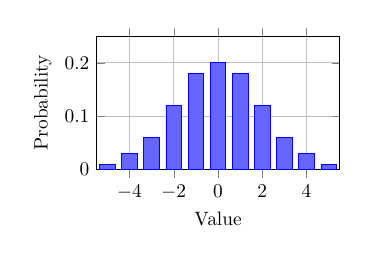
\begin{tikzpicture}[scale=0.7]
					\begin{axis}[
							ybar,
							bar width=8pt,
							xlabel={Value},
							ylabel={Probability},
							ymin=0, ymax=0.25,
							xmin=-5.5, xmax=5.5,
							xtick={-4,-2,0,2,4},
							width=6cm,
							height=4cm,
							grid=major,
						]
						\addplot[fill=blue!60,draw=blue] coordinates {
								(-5,0.01) (-4,0.03) (-3,0.06) (-2,0.12) (-1,0.18)
								(0,0.20) (1,0.18) (2,0.12) (3,0.06) (4,0.03) (5,0.01)
							};
					\end{axis}
				\end{tikzpicture}
				\\
				\textbf{Uniform}\\[2mm]
				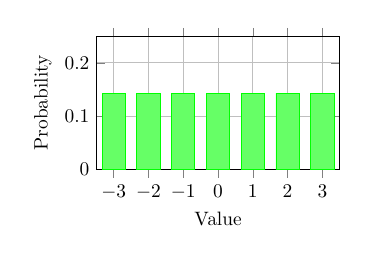
\begin{tikzpicture}[scale=0.7]
					\begin{axis}[
							ybar,
							bar width=12pt,
							xlabel={Value},
							ylabel={Probability},
							ymin=0, ymax=0.25,
							xmin=-3.5, xmax=3.5,
							xtick={-3,-2,-1,0,1,2,3},
							width=6cm,
							height=4cm,
							grid=major,
						]
						\addplot[fill=green!60,draw=green] coordinates {
								(-3,0.143) (-2,0.143) (-1,0.143) (0,0.143)
								(1,0.143) (2,0.143) (3,0.143)
							};
					\end{axis}
				\end{tikzpicture}
			\end{center}
		\end{column}
	\end{columns}
\end{frame}

\begin{frame}{Key Agreement vs Key Encapsulation}
	\begin{columns}[c]
		\begin{column}{0.5\textwidth}
			\textbf{Shared Secret Agreement (DH-style):}
			\begin{itemize}
				\item Both parties contribute randomness
				\item Alice: $g^a$, Bob: $g^b$
				\item Shared secret: $g^{ab}$
				\item \textbf{Interactive}: Both parties actively compute
				\item Traditional approach (RSA, ECDH)
			\end{itemize}
		\end{column}
		\begin{column}{0.5\textwidth}
			\textbf{Key Encapsulation (KEM):}
			\begin{itemize}
				\item One party generates the key
				\item Alice: Generates random key $k$
				\item Alice: Encapsulates $k$ \rightarrow\ ciphertext $c$
				\item Bob: Decapsulates $c$ \rightarrow\ key $k$
				\item \textbf{Asymmetric}: One generates, one recovers
			\end{itemize}
		\end{column}
	\end{columns}
	\vspace{5mm}
	\begin{center}
		\textbf{Both achieve the same goal}: Establish a shared secret key
	\end{center}
\end{frame}

\begin{frame}{From LWE to key encapsulation}
	\begin{itemize}
		\item \textbf{Key insight}: LWE naturally supports key encapsulation mechanisms (KEMs)
		\item \textbf{KEM approach}: One party generates and encapsulates a key
		\item \textbf{Recipient}: Uses private key to decapsulate and recover the key
		\item \textbf{Why KEMs?}:
		      \begin{itemize}
			      \item Lattice problems don't naturally support DH-style operations
			      \item No efficient ``commutative'' operation like $g^{ab} = g^{ba}$
			      \item KEMs are the natural construction for lattice-based crypto
		      \end{itemize}
		\item \textbf{Reconciliation}: Still needed to extract identical keys from noisy values
	\end{itemize}
\end{frame}

\begin{frame}{Mathematical notation primer}
	\begin{itemize}
		\item \textbf{Vectors}: Written with arrows, e.g., $\vec{s}$, $\vec{r}$
		      \begin{itemize}
			      \item A vector is a list of numbers: $\vec{s} = \begin{bmatrix} s_1 \\ s_2 \\ \vdots \\ s_n \end{bmatrix}$
			      \item Length $n$ vector has $n$ components
		      \end{itemize}
		\item \textbf{Matrices}: 2D arrays of numbers, e.g., $A \in \mathbb{Z}_q^{n \times n}$
		      \begin{itemize}
			      \item $n \times n$ means $n$ rows and $n$ columns
			      \item $\mathbb{Z}_q$ means integers modulo $q$ (from 0 to $q-1$)
		      \end{itemize}
		\item \textbf{Matrix transpose}: Flip rows and columns
		      \begin{itemize}
			      \item If $A = \begin{bmatrix} 1 & 2 \\ 3 & 4 \end{bmatrix}$, then $A^T = \begin{bmatrix} 1 & 3 \\ 2 & 4 \end{bmatrix}$
			      \item For vectors: $\vec{v}^T$ turns a column into a row
		      \end{itemize}
	\end{itemize}
\end{frame}

\begin{frame}{Sampling and distribution notation}
	\begin{columns}[c]
		\begin{column}{0.5\textwidth}
			\textbf{Sampling notation:}
			\begin{itemize}
				\item $x \twoheadleftarrow S$ means ``randomly pick $x$ from set $S$''
				\item Like rolling dice or drawing from a hat
			\end{itemize}
			\vspace{3mm}
			\textbf{Error distribution $\mathcal{E}$:}
			\begin{itemize}
				\item A probability distribution over small integers
			\end{itemize}
		\end{column}
		\begin{column}{0.5\textwidth}
			\textbf{Sampling examples:}
			\begin{itemize}
				\item $e \twoheadleftarrow \mathcal{E}$
				      \begin{itemize}
					      \item Sample one small integer
					      \item Result: e.g., $e = -1$
				      \end{itemize}
				\item $\vec{e} \twoheadleftarrow [\mathcal{E}]^n$
				      \begin{itemize}
					      \item Sample $n$ integers independently
					      \item Result: e.g., $\vec{e} = \begin{bmatrix} 0 \\ 1 \\ -1 \\ 0 \end{bmatrix}$
				      \end{itemize}
			\end{itemize}
		\end{column}
	\end{columns}
\end{frame}

\begin{frame}{Other notation in the KEM}
	\begin{itemize}
		\item \textbf{Floor function}: $\lfloor x \rfloor$ means round down to nearest integer
		      \begin{itemize}
			      \item $\lfloor 3.7 \rfloor = 3$, $\lfloor 5.1 \rfloor = 5$
			      \item $\lfloor q/2 \rfloor$ = halfway point in $\mathbb{Z}_q$
			      \item If $q = 3329$, then $\lfloor q/2 \rfloor = 1664$
		      \end{itemize}
		\item \textbf{Matrix-vector multiplication}:
		      \begin{itemize}
			      \item $A\vec{s}$: Matrix $A$ times vector $\vec{s}$ gives a vector
			      \item $\vec{b}^T\vec{r}$: Row vector times column vector gives a scalar (number)
		      \end{itemize}
		\item \textbf{The shared bit $\mu$}:
		      \begin{itemize}
			      \item The actual message being transmitted: 0 or 1
			      \item Encoded by adding 0 (if $\mu = 0$) or $\lfloor q/2 \rfloor$ (if $\mu = 1$)
			      \item Small errors won't confuse 0 with $\lfloor q/2 \rfloor$
		      \end{itemize}
	\end{itemize}
\end{frame}

\begin{frame}{Simple LWE-based KEM}
	\begin{columns}[c]
		\begin{column}{0.5\textwidth}
			\textbf{Public parameters:}
			\begin{itemize}
				\item Matrix $A \in \mathbb{Z}_q^{n \times n}$
				\item Modulus $q$ (e.g., 3329)\footnote{3329 is congruent to 1 modulo 256, and therefore the polynomial $X^{256} + 1$ splits into a product of degreen $2$ polynomials of the form $(X^2 - r_{i}).$}\footnote{\url{https://appliedcryptography.page/paper/\#basic-lattice}}
				\item Error distribution $\mathcal{E}$
			\end{itemize}
			\textbf{Bob's key generation:}
			\begin{enumerate}
				\item Sample $(\vec{s}, \vec{e}_1) \twoheadleftarrow [\mathcal{E}]^n$
				\item Private key: $\vec{s}$
				\item Public key: $\vec{b} = A\vec{s} + \vec{e}_1$
				\item Publish $(A, \vec{b})$
			\end{enumerate}
		\end{column}
		\begin{column}{0.5\textwidth}
			\textbf{Alice's encapsulation:}
			\begin{enumerate}
				\item Sample $(\vec{r}, \vec{e}_2) \twoheadleftarrow [\mathcal{E}]^n$
				\item Sample $e_3 \twoheadleftarrow \mathcal{E}$
				\item Message bit: $\mu \in \bits$
				\item Compute:
				      \begin{itemize}
					      \item $\vec{u}^T = \vec{r}^{T}A + \vec{e}_{2}^{T}$
					      \item $v = \vec{r}^T\vec{t} + e_3 + \lfloor q/2 \rfloor \cdot \mu$
				      \end{itemize}
				\item Send ciphertext: $(\vec{u}, v)$
			\end{enumerate}
			\textbf{Bob's decapsulation:}
			\begin{enumerate}
				\item Compute: $w = v - \vec{u}^{T}\vec{s}$
				\item If $w$ closer to 0: $\mu = 0$
				\item If $w$ closer to $\lfloor q/2 \rfloor$: $\mu = 1$
			\end{enumerate}
		\end{column}
	\end{columns}
\end{frame}

\begin{frame}{Why decapsulation works}
	\begin{align*}
		v - \vec{u}^T\vec{s} & = \vec{r}^{T}(A\vec{s} + \vec{e}_1) + e_3 + \lfloor q/2 \rfloor \cdot \mu - (\vec{r}^{T}A + \vec{e}_{2}^{T})\vec{s}               \\
		                     & = \vec{r}^{T}A\vec{s} + \vec{r}^{T}\vec{e}_1 + e_3 + \lfloor q/2 \rfloor \cdot \mu - \vec{r}^{T}A\vec{s} - \vec{e}_{2}^{T}\vec{s} \\
		                     & = \vec{r}^{T}\vec{e}_{1} + e_3 + \lfloor q/2 \rfloor \cdot \mu - \vec{e}_{2}^{T}\vec{s}                                           \\
		                     & = \lfloor q/2 \rfloor \cdot \mu + \underbrace{(\vec{r}^{T}\vec{e}_{1} - \vec{e}_{2}^{T}\vec{s} + e_3)}_{\text{small error}}
	\end{align*}
\end{frame}

\begin{frame}{Why decapsulation works}
	\begin{columns}[c]
		\begin{column}{0.4\textwidth}
			\tiny
			\begin{align*}
				v - \vec{u}^T\vec{s} & = \vec{r}^{T}(A\vec{s} + \vec{e}_1) + e_3 + \lfloor q/2 \rfloor \cdot \mu - (\vec{r}^{T}A + \vec{e}_{2}^{T})\vec{s}               \\
				                     & = \vec{r}^{T}A\vec{s} + \vec{r}^{T}\vec{e}_1 + e_3 + \lfloor q/2 \rfloor \cdot \mu - \vec{r}^{T}A\vec{s} - \vec{e}_{2}^{T}\vec{s} \\
				                     & = \vec{r}^{T}\vec{e}_{1} + e_3 + \lfloor q/2 \rfloor \cdot \mu - \vec{e}_{2}^{T}\vec{s}                                           \\
				                     & = \lfloor q/2 \rfloor \cdot \mu + \underbrace{(\vec{r}^{T}\vec{e}_{1} - \vec{e}_{2}^{T}\vec{s} + e_3)}_{\text{small error}}
			\end{align*}
		\end{column}
		\begin{column}{0.6\textwidth}
			\begin{itemize}
				\item \textbf{Step 1}: Start with $v - \vec{u}^T\vec{s}$ and substitute the definitions
				      \begin{itemize}
					      \item Recall: $v = \vec{r}^T\vec{b} + e_3 + \lfloor q/2 \rfloor \cdot \mu$ where $\vec{b} = A\vec{s} + \vec{e}_1$
					      \item So: $v = \vec{r}^T(A\vec{s} + \vec{e}_1) + e_3 + \lfloor q/2 \rfloor \cdot \mu$
					      \item And: $\vec{u}^T = \vec{r}^TA + \vec{e}_2^T$
					      \item Substituting: $v - \vec{u}^T\vec{s} = \vec{r}^T(A\vec{s} + \vec{e}_1) + e_3 + \lfloor q/2 \rfloor \cdot \mu - (\vec{r}^TA + \vec{e}_2^T)\vec{s}$
				      \end{itemize}
				\item \textbf{Step 2}: Expand the products using distributivity
				      \begin{itemize}
					      \item $\vec{r}^T(A\vec{s} + \vec{e}_1) = \vec{r}^TA\vec{s} + \vec{r}^T\vec{e}_1$
					      \item $(\vec{r}^TA + \vec{e}_2^T)\vec{s} = \vec{r}^TA\vec{s} + \vec{e}_2^T\vec{s}$
					      \item Result: $\vec{r}^TA\vec{s} + \vec{r}^T\vec{e}_1 + e_3 + \lfloor q/2 \rfloor \cdot \mu - \vec{r}^TA\vec{s} - \vec{e}_2^T\vec{s}$
				      \end{itemize}
			\end{itemize}
		\end{column}
	\end{columns}
\end{frame}

\begin{frame}{Why decapsulation works}
	\begin{columns}[c]
		\begin{column}{0.4\textwidth}
			\tiny
			\begin{align*}
				v - \vec{u}^T\vec{s} & = \vec{r}^{T}(A\vec{s} + \vec{e}_1) + e_3 + \lfloor q/2 \rfloor \cdot \mu - (\vec{r}^{T}A + \vec{e}_{2}^{T})\vec{s}               \\
				                     & = \vec{r}^{T}A\vec{s} + \vec{r}^{T}\vec{e}_1 + e_3 + \lfloor q/2 \rfloor \cdot \mu - \vec{r}^{T}A\vec{s} - \vec{e}_{2}^{T}\vec{s} \\
				                     & = \vec{r}^{T}\vec{e}_{1} + e_3 + \lfloor q/2 \rfloor \cdot \mu - \vec{e}_{2}^{T}\vec{s}                                           \\
				                     & = \lfloor q/2 \rfloor \cdot \mu + \underbrace{(\vec{r}^{T}\vec{e}_{1} - \vec{e}_{2}^{T}\vec{s} + e_3)}_{\text{small error}}
			\end{align*}
		\end{column}
		\begin{column}{0.6\textwidth}
			\begin{itemize}
				\item \textbf{Step 3}: Cancel the $\vec{r}^TA\vec{s}$ terms
				      \begin{itemize}
					      \item Notice: $+\vec{r}^TA\vec{s}$ and $-\vec{r}^TA\vec{s}$ cancel out
					      \item Left with: $\vec{r}^T\vec{e}_1 + e_3 + \lfloor q/2 \rfloor \cdot \mu - \vec{e}_2^T\vec{s}$
				      \end{itemize}
				\item \textbf{Step 4}: Rearrange to isolate the message
				      \begin{itemize}
					      \item Group error terms: $\vec{r}^T\vec{e}_1 - \vec{e}_2^T\vec{s} + e_3$
					      \item Final form: $\lfloor q/2 \rfloor \cdot \mu + (\vec{r}^T\vec{e}_1 - \vec{e}_2^T\vec{s} + e_3)$
				      \end{itemize}
				\item \textbf{Why this works}:
				      \begin{itemize}
					      \item All error terms ($\vec{e}_1$, $\vec{e}_2$, $e_3$, $\vec{r}$, $\vec{s}$) are small
					      \item Their products and sums remain small
					      \item If $\mu = 0$: Result is close to 0
					      \item If $\mu = 1$: Result is close to $\lfloor q/2 \rfloor$
					      \item Small errors don't confuse these two cases!
				      \end{itemize}
			\end{itemize}
		\end{column}
	\end{columns}
\end{frame}

\begin{frame}{Reconciliation: Getting exact agreement}
	\begin{itemize}
		\item \textbf{Problem}: Noise might cause decapsulation errors
		\item \textbf{Solution}: Error correction codes or reconciliation mechanisms
		\item \textbf{Modern approach}:
		      \begin{enumerate}
			      \item Encode message bits with error correction
			      \item Add reconciliation data to help correct errors
			      \item Ensure Bob always recovers Alice's intended key
		      \end{enumerate}
		\item \textbf{Example} (simplified):
		      \begin{itemize}
			      \item Instead of single bit $\mu$, encode multiple bits
			      \item Use redundancy to correct small errors
			      \item Kyber uses sophisticated reconciliation for reliability
		      \end{itemize}
	\end{itemize}
\end{frame}

\begin{frame}{From theory to practice: Kyber}
	\begin{itemize}
		\item \textbf{CRYSTALS-Kyber}: NIST-standardized LWE-based KEM
		\item \textbf{Key improvements over basic scheme}:
		      \begin{itemize}
			      \item Uses structured matrices (polynomial rings) for efficiency
			      \item Module-LWE instead of plain LWE
			      \item Careful parameter selection for security/performance balance
			      \item CCA-secure construction using Fujisaki-Okamoto transform
		      \end{itemize}
		\item \textbf{Performance}: Competitive with current elliptic curve cryptography
		\item \textbf{Already deployed}: Chrome, Cloudflare, AWS, and others
	\end{itemize}
\end{frame}

\begin{frame}{The Fujisaki-Okamoto Transform}{Reminder}
	\begin{columns}[c]
		\begin{column}{0.6\textwidth}
			\begin{itemize}[<+->]
				\item Many public-key schemes (RSA, ElGamal) are only CPA-secure.
				\item The \textbf{Fujisaki-Okamoto (FO) transform} converts CPA-secure PKE to CCA-secure PKE.
				\item Basic idea:
				      \begin{itemize}
					      \item Use randomness derived from the message itself.
					      \item Add redundancy that can be verified during decryption.
					      \item Invalid ciphertexts will fail verification.
				      \end{itemize}
			\end{itemize}
		\end{column}
		\begin{column}{0.4\textwidth}
			\definitionbox{FO Transform (simplified)}{
				Given CPA-secure PKE scheme $\Pi$:
				\begin{itemize}
					\item $\texttt{Enc}_{FO}(pk, M)$:
					      \begin{enumerate}
						      \item $R \coloneq H(M)$
						      \item $C_1 \coloneq \Pi.\texttt{Enc}(pk, M; R)$
						      \item $C_2 \coloneq G(M) \oplus R'$
						      \item Return $(C_1, C_2)$
					      \end{enumerate}
					\item Decryption verifies consistency
				\end{itemize}
			}
		\end{column}
	\end{columns}
\end{frame}

\begin{frame}{LWE/Lattice-based crypto: The trade-offs}
	\begin{columns}[c]
		\begin{column}{0.5\textwidth}
			\textbf{Advantages:}
			\begin{itemize}
				\item[\mycheckmark] Fast operations
				\item[\mycheckmark] Both encryption \& signatures
				\item[\mycheckmark] NIST standardized
				\item[\mycheckmark] Efficient implementations
				\item[\mycheckmark] Flexible parameters
			\end{itemize}
		\end{column}
		\begin{column}{0.5\textwidth}
			\textbf{Disadvantages:}
			\begin{itemize}
				\item[$\times$] Newer assumptions (20 years)
				\item[$\times$] Larger than classical crypto
				\item[$\times$] Complex parameter selection
				\item[$\times$] Implementation pitfalls
			\end{itemize}
		\end{column}
	\end{columns}
	\vspace{5mm}
	\begin{center}
		\textbf{Bottom line}: Leading choice for general-purpose post-quantum cryptography
	\end{center}
\end{frame}

\subsection{Code-Based Cryptography}

\begin{frame}{Another PQ candidate: Code-based cryptography}
	\begin{itemize}
		\item \textbf{Different foundation}: Based on error-correcting codes
		\item \textbf{Long history}: Theory dates back to 1950s
		\item \textbf{Battle-tested}: McEliece cryptosystem (1978) still unbroken after 45+ years!
		\item \textbf{The trade-off}: Very secure, but public keys are large (100+ KB)
		\item \textbf{Modern perspective}: Is 100 KB really too big when average webpage is 2 MB?
	\end{itemize}
\end{frame}

\begin{frame}{What are error-correcting codes?}
	\begin{columns}[c]
		\begin{column}{0.7\textwidth}
			\begin{itemize}
				\item \textbf{The problem}: Transmitting data over noisy channels
				      \begin{itemize}
					      \item You send: \bit{010}
					      \item Channel flips a bit (hardware fault, solar flare\ldots)
					      \item Receiver gets: \bit{011} (wrong!)
				      \end{itemize}
				\item \textbf{The solution}: Add redundancy to detect and correct errors
				\item \textbf{Real-world applications}:
				      \begin{itemize}
					      \item CDs and DVDs (scratches don't destroy data)
					      \item Deep space communication (signals from Mars rovers)
					      \item QR codes (work even when partially damaged)
					      \item Computer memory (cosmic rays can flip bits!)
				      \end{itemize}
			\end{itemize}
		\end{column}
		\begin{column}{0.3\textwidth}
			\imagewithcaption{qr-code.png}{Thanks to error correction, this QR code will still work even if you cover \textit{any} small part of it with your hand. Try it!}
		\end{column}
	\end{columns}

\end{frame}

\begin{frame}{The simplest code: Repetition}
	\begin{columns}[c]
		\begin{column}{1\textwidth}
			\textbf{Basic idea}: Repeat each bit multiple times
			\begin{itemize}
				\item Original: \bit{010}
				\item Encoded: \bit{000 111 000}
				\item Each bit repeated 3 times
			\end{itemize}

			\textbf{Decoding}: Take majority vote
			\begin{itemize}
				\item Received: \bit{100 110 111}
				\item Decode: \bit{0} (two \bit{0}s) \bit{1} (two \bit{1}s) \bit{1} (three \bit{1}s)
				\item Result: \bit{011}
			\end{itemize}

			\textbf{Limitation}: Can only correct 1 error per 3-bit chunk
		\end{column}
	\end{columns}
\end{frame}

\begin{frame}{Linear codes: More sophisticated error correction}
	\begin{itemize}
		\item \textbf{Key idea}: Use linear algebra instead of simple repetition
		\item \textbf{Encoding process}:
		      \begin{enumerate}
			      \item Start with $n$-bit message vector $\vec{v}$
			      \item Multiply by generator matrix $G$ (size $m \times n$, where $m > n$)
			      \item Get codeword: $\vec{w} = \vec{v} \cdot G$
		      \end{enumerate}
		\item \textbf{The magic}: Matrix $G$ is designed so that:
		      \begin{itemize}
			      \item Codewords are spread far apart in ``code space''
			      \item Can correct up to $t$ errors (designer's choice)
			      \item More errors $\rightarrow$ larger codewords needed
		      \end{itemize}
		\item \textbf{Efficiency}: Much better than repetition codes!
	\end{itemize}
\end{frame}

\begin{frame}{Visualizing linear codes}
	\begin{center}
		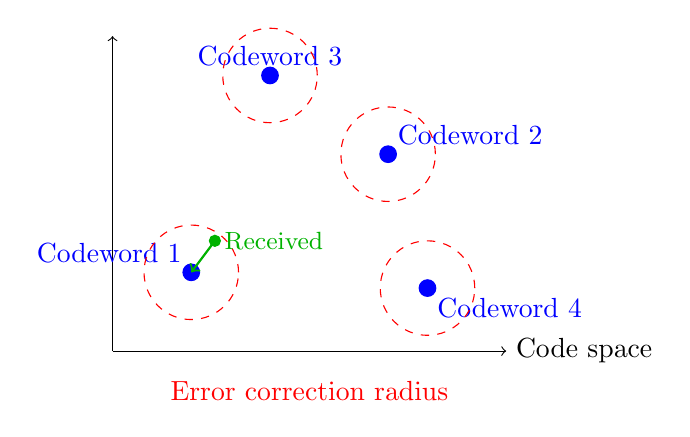
\begin{tikzpicture}[scale=1]
			\draw[->] (0,0) -- (5,0) node[right] {Code space};
			\draw[->] (0,0) -- (0,4);
			\filldraw[blue] (1,1) circle (3pt) node[above left] {Codeword 1};
			\filldraw[blue] (3.5,2.5) circle (3pt) node[above right] {Codeword 2};
			\filldraw[blue] (2,3.5) circle (3pt) node[above] {Codeword 3};
			\filldraw[blue] (4,0.8) circle (3pt) node[below right] {Codeword 4};
			\draw[dashed,red] (1,1) circle (0.6);
			\draw[dashed,red] (3.5,2.5) circle (0.6);
			\draw[dashed,red] (2,3.5) circle (0.6);
			\draw[dashed,red] (4,0.8) circle (0.6);
			\filldraw[green!70!black] (1.3,1.4) circle (2pt);
			\draw[->,green!70!black,thick] (1.3,1.4) -- (1,1);
			\node[green!70!black,right] at (1.3,1.4) {\small Received};
			\node[red] at (2.5,-0.5) {Error correction radius};
		\end{tikzpicture}
	\end{center}
	\begin{itemize}
		\item Codewords are far apart
		\item Errors move you within the ``sphere''
		\item Decode to nearest codeword
	\end{itemize}
\end{frame}

\begin{frame}{The McEliece cryptosystem (1978)}
	\begin{itemize}
		\item \textbf{Revolutionary idea}: Use error correction for encryption!
		\item \textbf{Public key}: Generator matrix $G = ABC$ (looks random)
		      \begin{itemize}
			      \item $A, B, C$ are special matrices (kept secret)
			      \item Product looks like random matrix
		      \end{itemize}
		\item \textbf{Encryption}:
		      \begin{enumerate}
			      \item Encode message: $\vec{w} = \vec{m} \cdot G$
			      \item Add controlled errors: $\vec{c} = \vec{w} + \vec{e}$
			      \item $\vec{e}$ has exactly $t$ bits set to 1
		      \end{enumerate}
		\item \textbf{Decryption}: Only possible if you know $A, B, C$
		      \begin{itemize}
			      \item Use secret structure to remove errors
			      \item Recover original message
		      \end{itemize}
	\end{itemize}
\end{frame}

\begin{frame}{Why is McEliece secure?}
	\begin{itemize}
		\item \textbf{The underlying problem}: Decoding random linear codes
		      \begin{itemize}
			      \item Given: Random-looking matrix and noisy codeword
			      \item Find: Original message
			      \item This is NP-hard! (No efficient algorithm known)
		      \end{itemize}
		\item \textbf{Quantum resistance}:
		      \begin{itemize}
			      \item No quantum algorithm gives significant speedup
			      \item Unlike factoring (Shor's algorithm)
			      \item 45+ years of cryptanalysis, still secure
		      \end{itemize}
		\item \textbf{Important caveat}: Not all instances of NP-hard problems are hard
		      \begin{itemize}
			      \item Need careful parameter selection
			      \item Decades of research have refined secure choices
		      \end{itemize}
	\end{itemize}
\end{frame}

\begin{frame}{Code-based crypto: Pros and cons}
	\begin{columns}[c]
		\begin{column}{0.5\textwidth}
			\textbf{Advantages:}
			\begin{itemize}
				\item[\mycheckmark] Long history (45+ years)
				\item[\mycheckmark] Well-understood security
				\item[\mycheckmark] Fast operations
				\item[\mycheckmark] Simple to implement
				\item[\mycheckmark] Quantum resistant
			\end{itemize}
		\end{column}
		\begin{column}{0.5\textwidth}
			\textbf{Disadvantages:}
			\begin{itemize}
				\item[$\times$] Large public keys (100+ KB)
				\item[$\times$] Not selected by NIST (yet)
				\item[$\times$] Less deployment experience
			\end{itemize}

			\vspace{5mm}
			\textbf{Perspective}: Is 100 KB really too big today?
		\end{column}
	\end{columns}
\end{frame}

\subsection{Hash-Based Cryptography}

\begin{frame}{Hash-based cryptography: A different approach}
	\begin{itemize}
		\item \textbf{Fundamental difference}: Not based on hard mathematical problems!
		\item \textbf{Instead}: Based on security of cryptographic hash functions
		\item \textbf{Key insight}: Quantum computers don't break hash functions
		      \begin{itemize}
			      \item No known quantum algorithm for finding collisions
			      \item No quantum speedup for finding preimages (beyond Grover's)
		      \end{itemize}
		\item \textbf{Security foundation}: If you can't invert hashes, you can't forge signatures
		\item \textbf{History}: Ideas date back to 1979 (Lamport, Winternitz)
	\end{itemize}
\end{frame}

\begin{frame}{The building block: One-time signatures}
	\begin{itemize}
		\item \textbf{One-time signature}: Can sign only ONE message with each key
		\item \textbf{Why accept this limitation?}
		      \begin{itemize}
			      \item Extremely simple construction
			      \item Provably secure (if hash is secure)
			      \item Building block for multi-use schemes
		      \end{itemize}
		\item \textbf{Real-world analogy}: Like a wax seal
		      \begin{itemize}
			      \item Break the seal to verify authenticity
			      \item Can't reuse it for another letter
			      \item Need a new seal for each message
		      \end{itemize}
	\end{itemize}
\end{frame}

\begin{frame}{Winternitz One-Time Signature (WOTS)}
	\begin{columns}[c]
		\begin{column}{1\textwidth}
			\textbf{Setup (for messages 0 to $w-1$):}
			\begin{itemize}
				\item Private key: Random string $K$
				\item Public key: $\text{Hash}^w(K)$
				      \begin{itemize}
					      \item Apply hash $w$ times
				      \end{itemize}
			\end{itemize}

			\textbf{To sign message $M$:}
			\begin{itemize}
				\item Signature: $\text{Hash}^M(K)$
				\item Apply hash $M$ times to $K$
			\end{itemize}
		\end{column}
	\end{columns}
\end{frame}

\begin{frame}{WOTS verification: Why it works}
	\begin{itemize}
		\item \textbf{Given}: Signature $S = \text{Hash}^M(K)$ for message $M$
		\item \textbf{Verification}: Check if $\text{Hash}^{w-M}(S) = \text{Public Key}$
		\item \textbf{Why this works}:
		      \begin{align*}
			      \text{Hash}^{w-M}(S) & = \text{Hash}^{w-M}(\text{Hash}^M(K)) \\
			                           & = \text{Hash}^{(w-M)+M}(K)            \\
			                           & = \text{Hash}^w(K)                    \\
			                           & = \text{Public Key} \mycheckmark
		      \end{align*}
		\item \textbf{Security}: Can't go backwards in the hash chain!
		      \begin{itemize}
			      \item Given $\text{Hash}^5(K)$, can't compute $\text{Hash}^3(K)$
			      \item Would require inverting the hash function
		      \end{itemize}
	\end{itemize}
\end{frame}

\begin{frame}{WOTS limitation 1: Signature forgery}
	\begin{itemize}
		\item \textbf{Critical flaw}: Can forge signatures for larger messages!
		\item \textbf{Example}:
		      \begin{itemize}
			      \item You sign message $M = 3$: $S = \text{Hash}^3(K)$
			      \item Attacker computes: $\text{Hash}(S) = \text{Hash}^4(K)$
			      \item This is a valid signature for message $M = 4$!
		      \end{itemize}
		\item \textbf{General attack}: From signature of $M$, can forge any $M' > M$
		\item \textbf{Fix}: Sign both $M$ and $w-M$ using two keys
		      \begin{itemize}
			      \item Signature: $(\text{Hash}^M(K_1), \text{Hash}^{w-M}(K_2))$
			      \item Now increasing $M$ requires decreasing $w-M$
			      \item But you can't go backwards in hash chains!
		      \end{itemize}
	\end{itemize}
\end{frame}

\begin{frame}{WOTS limitation 2: Message length}
	\begin{columns}[c]
		\begin{column}{0.55\textwidth}
			\textbf{The problem with long messages:}
			\begin{itemize}
				\item 8-bit message: $M \in [0, 255]$
				      \begin{itemize}
					      \item Need up to 255 hash operations
					      \item Manageable
				      \end{itemize}
				\item 32-bit message: $M \in [0, 2^{32}-1]$
				      \begin{itemize}
					      \item Need up to 4 billion hashes!
					      \item Impractical
				      \end{itemize}
				\item 128-bit message: $M \in [0, 2^{128}-1]$
				      \begin{itemize}
					      \item Need up to $2^{128}$ hashes
					      \item Impossible
				      \end{itemize}
			\end{itemize}
		\end{column}
		\begin{column}{0.45\textwidth}
			\textbf{Solution}: Split into chunks
			\begin{itemize}
				\item Break 32-bit message into four 8-bit chunks
				\item Sign each chunk independently
				\item Need 4 key pairs instead of 1
				\item Maximum 255 hashes per chunk
			\end{itemize}

			\textbf{Trade-off}:
			\begin{itemize}
				\item More keys = larger signatures
				\item But computation stays feasible
			\end{itemize}
		\end{column}
	\end{columns}
\end{frame}

\begin{frame}{WOTS limitation 3: The one-time problem}
	\begin{itemize}
		\item \textbf{Critical security requirement}: Never reuse a key!
		\item \textbf{What happens if you sign two messages?}
		      \begin{itemize}
			      \item Sign $M_1 = 2$: Reveal $\text{Hash}^2(K)$
			      \item Sign $M_2 = 7$: Reveal $\text{Hash}^7(K)$
			      \item Attacker can now compute $\text{Hash}^x(K)$ for any $x \in [2,7]$
			      \item Can forge signatures for messages 3, 4, 5, 6!
		      \end{itemize}
		\item \textbf{With the two-key fix}: Even worse
		      \begin{itemize}
			      \item Multiple signatures reveal different points on both chains
			      \item Attacker gains more forgery capabilities
		      \end{itemize}
		\item \textbf{No simple fix}: This is inherent to the construction
	\end{itemize}
\end{frame}

\begin{frame}{From one-time to many-time: Merkle trees}
	\begin{columns}[c]
		\begin{column}{0.5\textwidth}
			\textbf{The idea}: Use many OTS keys
			\begin{itemize}
				\item Generate $2^h$ one-time key pairs
				\item Build a Merkle tree of public keys
				\item Tree root = master public key
				\item Each leaf = one signature
			\end{itemize}

			\textbf{To sign}:
			\begin{itemize}
				\item Use next unused OTS key
				\item Include path to root as proof
				\item Mark key as used (stateful!)
			\end{itemize}
		\end{column}
		\begin{column}{0.5\textwidth}
			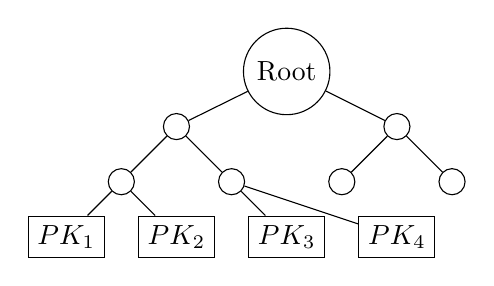
\begin{tikzpicture}[scale=0.7]
				\node[draw,circle] (root) at (4,3) {Root};
				\node[draw,circle] (n1) at (2,2) {};
				\node[draw,circle] (n2) at (6,2) {};
				\node[draw,circle] (n3) at (1,1) {};
				\node[draw,circle] (n4) at (3,1) {};
				\node[draw,circle] (n5) at (5,1) {};
				\node[draw,circle] (n6) at (7,1) {};
				\node[draw,rectangle] (pk1) at (0,0) {$PK_1$};
				\node[draw,rectangle] (pk2) at (2,0) {$PK_2$};
				\node[draw,rectangle] (pk3) at (4,0) {$PK_3$};
				\node[draw,rectangle] (pk4) at (6,0) {$PK_4$};

				\draw (root) -- (n1);
				\draw (root) -- (n2);
				\draw (n1) -- (n3);
				\draw (n1) -- (n4);
				\draw (n2) -- (n5);
				\draw (n2) -- (n6);
				\draw (n3) -- (pk1);
				\draw (n3) -- (pk2);
				\draw (n4) -- (pk3);
				\draw (n4) -- (pk4);
			\end{tikzpicture}
		\end{column}
	\end{columns}
\end{frame}

\begin{frame}{Modern hash-based signatures}
	\begin{itemize}
		\item \textbf{XMSS (eXtended Merkle Signature Scheme)}:
		      \begin{itemize}
			      \item Stateful: Must track which keys are used
			      \item Smaller signatures than SPHINCS+
			      \item Risk: Reusing state breaks security
		      \end{itemize}
		\item \textbf{SPHINCS+ (NIST standard: SLH-DSA)}:
		      \begin{itemize}
			      \item Stateless: No need to track used keys
			      \item Larger signatures (tens of KB)
			      \item Uses sophisticated tree structures
			      \item ``Few-time'' signatures instead of one-time
		      \end{itemize}
		\item \textbf{Key limitation}: Signatures only!
		      \begin{itemize}
			      \item Hash functions are one-way
			      \item Can't build encryption from one-way functions alone
		      \end{itemize}
	\end{itemize}
\end{frame}

\begin{frame}{Hash-based crypto: The trade-offs}
	\begin{columns}[c]
		\begin{column}{0.5\textwidth}
			\textbf{Advantages:}
			\begin{itemize}
				\item[\mycheckmark] Simplest security assumption
				\item[\mycheckmark] Well-understood (40+ years)
				\item[\mycheckmark] Quantum resistant
				\item[\mycheckmark] Fast verification
				\item[\mycheckmark] Can be stateless
			\end{itemize}
		\end{column}
		\begin{column}{0.5\textwidth}
			\textbf{Disadvantages:}
			\begin{itemize}
				\item[$\times$] Large signatures (10-50 KB)
				\item[$\times$] Signatures only (no encryption)
				\item[$\times$] Complex key generation
				\item[$\times$] Stateful variants risky
			\end{itemize}
		\end{column}
	\end{columns}
	\vspace{5mm}
	\begin{center}
		\textbf{Bottom line}: Most conservative choice for long-term signatures
	\end{center}
\end{frame}

\section{Today's Post-Quantum Protocols}

\begin{frame}{Moving towards the middle}
	\bigimagewithcaption{fischer.png}{Fischer et al., The Challenges of Bringing Cryptography from Research Papers to Products: Results from an Interview Study with Experts, USENIX Security 2024}
\end{frame}

\begin{frame}{NIST PQ standardization: The winners}
	\begin{itemize}
		\item \textbf{August 2024}: NIST released final standards after 8-year process
		\item \textbf{Three primary standards} (with new names):
	\end{itemize}

	\begin{center}
		\begin{tabular}{|l|l|l|}
			\hline
			\textbf{Original Name} & \textbf{Standard Name} & \textbf{Hard Problem} \\
			\hline
			\hline
			\multicolumn{3}{|c|}{\textit{Key Encapsulation}}                        \\
			\hline
			CRYSTALS-Kyber         & ML-KEM                 & Module LWE            \\
			\hline
			\hline
			\multicolumn{3}{|c|}{\textit{Digital Signatures}}                       \\
			\hline
			CRYSTALS-Dilithium     & ML-DSA                 & Module LWE            \\
			FALCON                 & FN-DSA                 & NTRU lattice          \\
			SPHINCS+               & SLH-DSA                & Hash functions        \\
			\hline
		\end{tabular}
	\end{center}

	\begin{itemize}
		\item \textbf{ML}: Module Lattice
		\item \textbf{FN}: Fast Fourier transform over NTRU
		\item \textbf{SLH}: Stateless Hash-based
	\end{itemize}
\end{frame}

\begin{frame}{Key Agreement vs Key Encapsulation}
	\begin{columns}[c]
		\begin{column}{0.5\textwidth}
			\textbf{Shared Secret Agreement (DH-style):}
			\begin{itemize}
				\item Both parties contribute randomness
				\item Alice: $g^a$, Bob: $g^b$
				\item Shared secret: $g^{ab}$
				\item \textbf{Interactive}: Both parties actively compute
				\item Traditional approach (RSA, ECDH)
			\end{itemize}
		\end{column}
		\begin{column}{0.5\textwidth}
			\textbf{Key Encapsulation (KEM):}
			\begin{itemize}
				\item One party generates the key
				\item Alice: Generates random key $k$
				\item Alice: Encapsulates $k$ \rightarrow\ ciphertext $c$
				\item Bob: Decapsulates $c$ \rightarrow\ key $k$
				\item \textbf{Asymmetric}: One generates, one recovers
			\end{itemize}
		\end{column}
	\end{columns}
	\vspace{5mm}
	\begin{center}
		\textbf{Both achieve the same goal}: Establish a shared secret key
	\end{center}
\end{frame}

\begin{frame}{KEMs use public/private key pairs}
	\begin{itemize}
		\item \textbf{KEMs still use asymmetric cryptography}:
		      \begin{itemize}
			      \item Bob has a public/private key pair $(pk_B, sk_B)$
			      \item Bob's public key is shared openly
			      \item Bob's private key is kept secret
		      \end{itemize}
		\item \textbf{The KEM process}:
		      \begin{enumerate}
			      \item Alice obtains Bob's public key $pk_B$
			      \item Alice generates random shared secret $k$
			      \item Alice encapsulates: $c = \text{Encaps}(pk_B, k)$
			      \item Alice sends ciphertext $c$ to Bob
			      \item Bob decapsulates: $k = \text{Decaps}(sk_B, c)$
		      \end{enumerate}
		\item \textbf{Security guarantee}: Only Bob (with $sk_B$) can recover $k$ from $c$
	\end{itemize}
\end{frame}

\begin{frame}{Why KEMs for Post-Quantum?}{Why not do shared secret agreement like Diffie-Hellman?}
	\begin{itemize}
		\item \textbf{Efficiency with lattices/codes}:
		      \begin{itemize}
			      \item Natural fit: ``Encrypt'' a random key with public key
			      \item Avoid complex reconciliation mechanisms
			      \item Better bandwidth usage
			      \item Potentially less round trips
		      \end{itemize}
		\item \textbf{Mathematical limitations}:
		      \begin{itemize}
			      \item Lattice problems don't naturally support DH-style operations
			      \item No efficient ``commutative'' group operation like $g^{ab} = g^{ba}$
			      \item Isogenies do support DH-style, but have other issues
		      \end{itemize}
		\item \textbf{NIST's choice (rumored)}:
		      \begin{itemize}
			      \item KEMs work for all mathematical foundations
			      \item Unified framework for competition
			      \item Avoids favoring specific mathematical structures
		      \end{itemize}
	\end{itemize}
\end{frame}

\begin{frame}{X-Wing: An optimized hybrid KEM}
	\begin{columns}[c]
		\begin{column}{1\textwidth}
			\begin{itemize}
				\item \textbf{What is X-Wing?}
				      \begin{itemize}
					      \item Purpose-built hybrid KEM combining X25519 and ML-KEM-768\footnote{\url{https://appliedcryptography.page/paper/\#xwing-hybrid}}
					      \item Designed to be ``the sensible choice for most applications''
				      \end{itemize}
				\item \textbf{Efficiency gains}:
				      \begin{itemize}
					      \item Tailored construction beats generic KEM combiners
					      \item Takes advantage of specific properties of X25519 and ML-KEM-768
				      \end{itemize}
				\item \textbf{Security guarantees}:
				      \begin{itemize}
					      \item Secure if \textbf{either} X25519 OR ML-KEM-768 remains secure
					      \item Classical security: IND-CCA if strong DH holds (proven in ROM)
					      \item Post-quantum security: IND-CCA if ML-KEM-768 is IND-CCA (standard model)
				      \end{itemize}
				\item Concrete choices enable both optimizations and stronger proofs!
			\end{itemize}
		\end{column}
	\end{columns}
\end{frame}

\subsection{Post-Quantum TLS}

\begin{frame}{TLS migration timeline}
	\begin{columns}[c]
		\begin{column}{1\textwidth}
			\begin{itemize}
				\item \textbf{February 2024}: PQ TLS 1.3 adoption reaches critical mass\footnote{Much of the slides in this subsection are based on Bas Westerbaan's excellent blog post over at Cloudflare, but have been updated to account for developments in 2024 and 2025: \url{https://blog.cloudflare.com/pq-2024/}}
				\item \textbf{QUIC protocol}: Uses TLS 1.3 under the hood
				      \begin{itemize}
					      \item Modern transport protocol by Google
					      \item Built-in encryption via TLS 1.3
					      \item Already quantum-ready infrastructure
				      \end{itemize}
				\item \textbf{Preventing future ossification}: GREASE
				      \begin{itemize}
					      \item Generate Random Extensions And Sustain Extensibility
					      \item Clients send unknown identifiers on purpose
					      \item Catches implementations that break on unknown values
					      \item Keeps protocols flexible for future changes
				      \end{itemize}
			\end{itemize}
		\end{column}
	\end{columns}
\end{frame}

\begin{frame}{ML-KEM: The NIST standard}
	\begin{itemize}
		\item \textbf{Original name}: CRYSTALS-Kyber
		\item \textbf{International collaboration}:
		      \begin{itemize}
			      \item Designers from France, Switzerland, Netherlands, Belgium, Germany, Canada, USA
			      \item Industry and academia partnership
		      \end{itemize}
		\item \textbf{Three security levels}:
		      \begin{itemize}
			      \item ML-KEM-512: Targets AES-128 equivalent security
			      \item ML-KEM-768: Targets AES-192 equivalent security
			      \item ML-KEM-1024: Targets AES-256 equivalent security
		      \end{itemize}
		\item \textbf{First NIST PQ key agreement standard}
	\end{itemize}
\end{frame}

\begin{frame}{ML-KEM vs X25519 (ECDH): The numbers}
	\begin{center}
		\begin{tabular}{|l|c|c|c|c|c|}
			\hline
			\textbf{Algorithm} & \textbf{PQ}  & \multicolumn{2}{c|}{\textbf{Size (bytes)}} & \multicolumn{2}{c|}{\textbf{Ops/sec}}                   \\
			                   &              & Client                                     & Server                                & Client & Server \\
			\hline
			ML-KEM-512         & \mycheckmark & 800                                        & 768                                   & 45,000 & 70,000 \\
			ML-KEM-768         & \mycheckmark & 1,184                                      & 1,088                                 & 29,000 & 45,000 \\
			ML-KEM-1024        & \mycheckmark & 1,568                                      & 1,568                                 & 20,000 & 30,000 \\
			X25519             & \times       & 32                                         & 32                                    & 19,000 & 19,000 \\
			\hline
		\end{tabular}
	\end{center}
	\vspace{3mm}
	\begin{itemize}
		\item \textbf{Size penalty}: ML-KEM is 25-50\times\ larger than X25519
		\item \textbf{Speed bonus}: ML-KEM can be faster
		\item \textbf{Trade-off}: Bandwidth vs computation
	\end{itemize}
\end{frame}

\begin{frame}{Hybrid key agreement: Belt and suspenders}
	\textbf{Common deployment}: X25519 + ML-KEM-768
	\vspace{3mm}
	\begin{columns}[c]
		\begin{column}{0.5\textwidth}
			\textbf{Why ML-KEM-768?}
			\begin{itemize}
				\item Not just ML-KEM-512
				\item Security margin against future cryptanalysis
				\item Lattice crypto is newer than elliptic curves
				\item Conservative choice
			\end{itemize}
		\end{column}
		\begin{column}{0.5\textwidth}
			\textbf{Why keep X25519?}
			\begin{itemize}
				\item Hedge against ML-KEM break
				\item Protection against implementation bugs
				\item Example: KyberSlash timing attack
				\item Proven track record
			\end{itemize}
		\end{column}
	\end{columns}
	\vspace{5mm}
	\begin{center}
		\textbf{Result}: Security of both, vulnerable only if both break
	\end{center}
\end{frame}

\begin{frame}{Early browser experiments}
	\begin{columns}[c]
		\begin{column}{1\textwidth}
			\begin{itemize}
				\item \textbf{2016}: Google's first PQ experiment (same year as NIST competition)
				\item \textbf{2018}: Cloudflare + Google joint experiment
				      \begin{itemize}
					      \item CECPQ2: X25519 + NTRU-HRSS (lattice-based)
					      \item CECPQ2b: X25519 + SIKE (isogeny-based)
				      \end{itemize}
				\item \textbf{Results}:
				      \begin{itemize}
					      \item NTRU-HRSS: Good performance, similar to ML-KEM
					      \item SIKE: Small keys but slow, \textcolor{red}{completely broken in 2022}
					            \begin{itemize}
						            \item Good argument for hybrid cryptosystems (like X-Wing\footnote{\url{https://appliedcryptography.page/paper/\#xwing-hybrid}}) that combine both classical and PQ crypto!
					            \end{itemize}
					      \item Handshake times nearly identical to classical crypto
				      \end{itemize}
				\item \textbf{But}: Compatibility issues emerged\ldots
			\end{itemize}
		\end{column}
	\end{columns}
\end{frame}

\begin{frame}{The ClientHello size problem}
	\begin{columns}[c]
		\begin{column}{0.6\textwidth}
			\textbf{The ossification strikes again:}
			\begin{itemize}
				\item TLS ClientHello historically fit in one packet
				\item PQ keyshares make it much larger
				\item Some middleboxes assume single-packet ClientHello
				\item Result: Broken connections
			\end{itemize}

			\textbf{Chrome's response:}
			\begin{itemize}
				\item Kept PQ experiment at low rate
				\item Worked with vendors to fix issues
				\item 5-year delay in deployment
			\end{itemize}
		\end{column}
		\begin{column}{0.4\textwidth}
			\begin{center}
				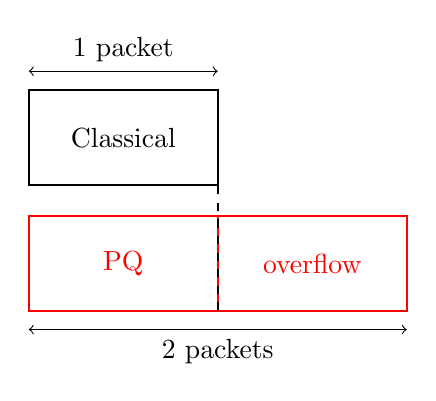
\begin{tikzpicture}[scale=0.8]
					\draw[thick] (0,0) rectangle (3,1.5) node[midway] {Classical};
					\draw[thick,red] (0,-2) rectangle (3,-0.5) node[midway] {PQ};
					\draw[thick,red] (3,-2) rectangle (6,-0.5) node[midway] {overflow};
					\draw[<->] (0,1.8) -- (3,1.8) node[midway,above] {1 packet};
					\draw[<->] (0,-2.3) -- (6,-2.3) node[midway,below] {2 packets};
					\draw[thick,dashed] (3,-2) -- (3,1);
				\end{tikzpicture}
			\end{center}
		\end{column}
	\end{columns}
\end{frame}

\begin{frame}{Current deployment status (2025)}
	\begin{columns}[c]
		\begin{column}{0.6\textwidth}
			\textbf{Browsers have begun implementing PQ TLS:}
			\begin{itemize}
				\item Started with Chrome, now others following
				\item In total, now 38\% of all TLS connection\footnote{\url{https://radar.cloudflare.com/adoption-and-usage\#post-quantum-encryption-adoption}}
			\end{itemize}
			\textbf{Other browsers:}
			\begin{itemize}
				\item Firefox: since mid-2024
				\item Edge, Brave: based on Chrome, so followed it
				\item Safari: timeline announced at WWDC 2025\footnote{\url{https://support.apple.com/en-us/122756}} for iOS 26, macOS 26, etc.
			\end{itemize}
		\end{column}
		\begin{column}{0.4\textwidth}
			\begin{center}
				\textbf{PQ Adoption}\\[3mm]
				\begin{tikzpicture}[scale=0.8]
					\pie[text=legend,radius=2]{
						38/PQ,
						62/Classical
					}
				\end{tikzpicture}
			\end{center}
		\end{column}
	\end{columns}
\end{frame}

\begin{frame}{Beyond browsers: Origin connections}
	\begin{columns}[c]
		\begin{column}{1\textwidth}
			\textbf{The full connection path:}
			\begin{center}
				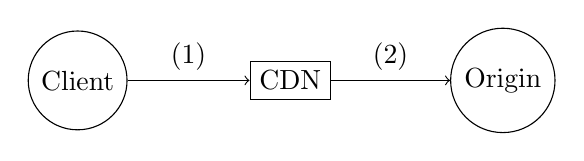
\begin{tikzpicture}[scale=0.9]
					\node[draw,circle] (client) at (0,0) {Client};
					\node[draw,rectangle] (cdn) at (3,0) {CDN};
					\node[draw,circle] (origin) at (6,0) {Origin};
					\draw[->] (client) -- (cdn) node[midway,above] {(1)};
					\draw[->] (cdn) -- (origin) node[midway,above] {(2)};
				\end{tikzpicture}
			\end{center}
			\textbf{Two approaches for CDN-to-origin PQ:}
			\begin{itemize}
				\item \textbf{Fast way}: Send PQ keyshare immediately
				      \begin{itemize}
					      \item Like Chrome's approach
					      \item 0.34\% connection failures observed
				      \end{itemize}
				\item \textbf{Safe way}: Wait for \texttt{HelloRetryRequest}
				      \begin{itemize}
					      \item Extra round trip
					      \item 100\% compatibility
				      \end{itemize}
			\end{itemize}
			\textbf{Failure causes}: Large \texttt{ClientHello} + incorrect \texttt{HelloRetryRequest} handling
		\end{column}
	\end{columns}
\end{frame}

\begin{frame}{Lessons from PQ TLS deployment}
	\begin{itemize}
		\item \textbf{Ossification is real}:
		      \begin{itemize}
			      \item Assumptions about packet sizes break deployments
			      \item GREASE helps but isn't perfect
			      \item Takes years to fix ecosystem
		      \end{itemize}
		\item \textbf{Hybrid approach is prudent}:
		      \begin{itemize}
			      \item Protects against algorithm breaks
			      \item Protects against implementation bugs
			      \item Small performance cost for peace of mind
		      \end{itemize}
		\item \textbf{Deployment is gradual}:
		      \begin{itemize}
			      \item Started in 2016, still ongoing in 2025
			      \item Requires coordination across entire ecosystem
			      \item But progress is accelerating
		      \end{itemize}
	\end{itemize}
\end{frame}

\subsection{Post-Quantum Secure Messaging}
% PQ3
\begin{frame}{Apple iMessage: PQ3}
	\bigimagewithcaption{pq3-apple.png}{Source: Apple Security Engineering and Architecture (SEAR)}
\end{frame}

\begin{frame}{iMessage PQ3: Post-quantum double ratchet}
	\begin{itemize}
		\item \textbf{PQ3}: Apple's post-quantum secure messaging protocol (2024)
		\item \textbf{Hybrid approach}: Combines classical (ECDH) and post-quantum (ML-KEM) cryptography
		\item \textbf{Double ratchet construction} (like Signal):
		      \begin{itemize}
			      \item Outer ratchet: Public-key ratchet (conversation direction changes)
			      \item Inner ratchet: Symmetric ratchet (same sender keeps sending)
		      \end{itemize}
		\item \textbf{Key innovation}: ML-KEM integrated into both initialization AND ratcheting
		      \begin{itemize}
			      \item Provides post-compromise security against quantum adversaries
			      \item Signal only uses PQ crypto in setup (PQXDH), not in ratcheting
		      \end{itemize}
		\item \textbf{Security guarantee}: Must break BOTH classical and PQ crypto to compromise
	\end{itemize}
\end{frame}

\begin{frame}{PQ3's bandwidth challenge: Ratcheting trade-offs}
	\begin{columns}[c]
		\begin{column}{0.55\textwidth}
			\textbf{The KEM size problem:}
			\begin{itemize}
				\item ML-KEM-768: 1,184 bytes sent
				\item ML-KEM-1024: 1,568 bytes sent
				\item Compare to X25519: 32 bytes!
			\end{itemize}
			\vspace{3mm}
			\textbf{PQ3's solution:}
			\begin{itemize}
				\item Can't send new KEM key with every message
				\item Heuristic: New KEM key every \approx50 messages
				\item Or at least once per week
				\item Trade-off: Less frequent PQ ratcheting
			\end{itemize}
		\end{column}
		\begin{column}{0.45\textwidth}
			\textbf{Signal (classical):}
			\begin{itemize}
				\item Small DH keys (32 bytes)
				\item Can ratchet with \textit{every} message
				\item Immediate post-compromise recovery
			\end{itemize}
			\vspace{3mm}
			\textbf{PQ3 (post-quantum):}
			\begin{itemize}
				\item Large KEM keys (1KB+)
				\item Ratchets every \approx50 messages
				\item Delayed post-compromise recovery
				\item But quantum-resistant!
			\end{itemize}
		\end{column}
	\end{columns}
\end{frame}

\begin{frame}{Signal: PQXDH for initial key agreement}
	\begin{itemize}
		\item \textbf{PQXDH}: Post-Quantum Extended Diffie-Hellman (2023)
		\item \textbf{Extends X3DH}: Signal's existing handshake protocol
		\item \textbf{Design goals}:
		      \begin{itemize}
			      \item Protect against store-now-decrypt-later (SNDL) attacks
			      \item No security loss compared to X3DH
			      \item Minimal changes to existing protocol
			      \item Efficient for Signal's usage patterns
		      \end{itemize}
		\item \textbf{Key insight}: Add PQ-KEM alongside existing DH operations
		      \begin{itemize}
			      \item Not replacing, but augmenting classical crypto
			      \item Hybrid approach for defense in depth
		      \end{itemize}
	\end{itemize}
\end{frame}

\begin{frame}{How PQXDH works}
	\begin{columns}[c]
		\begin{column}{0.55\textwidth}
			\textbf{X3DH (classical):}
			\begin{itemize}
				\item Multiple DH computations
				\item Identity keys (IK)
				\item Signed pre-keys (SPK)
				\item One-time pre-keys (OPK)
				\item Ephemeral keys (EK)
			\end{itemize}
			\vspace{3mm}
			\textbf{PQXDH additions:}
			\begin{itemize}
				\item \textcolor{blue}{+ KEM key pairs (PQSPK)}
				\item \textcolor{blue}{+ KEM encapsulation}
				\item \textcolor{blue}{+ Shared secret in KDF}
			\end{itemize}
		\end{column}
		\begin{column}{0.45\textwidth}
			\textbf{Protocol flow:}
			\begin{enumerate}
				\item Bob generates KEM keys
				\item Bob signs and uploads them
				\item Alice encapsulates to Bob's KEM key
				\item Both derive session key using:
				      \begin{itemize}
					      \item DH shared secrets
					      \item \textcolor{blue}{+ KEM shared secret}
				      \end{itemize}
			\end{enumerate}
			\vspace{3mm}
			\textbf{Result}: Key secure if either DH or KEM remains unbroken
		\end{column}
	\end{columns}
\end{frame}

\begin{frame}{How PQXDH works}
	\bigimagewithcaption{pqxdh-signal.png}{Source: \url{https://appliedcryptography.page/paper/\#pqxdh-analysis}}
\end{frame}

\begin{frame}{Lessons from PQXDH deployment}
	\begin{itemize}
		\item \textbf{Formal verification revealed issues}:
		      \begin{itemize}
			      \item Public key confusion attack (DH vs KEM keys)
			      \item KEM re-encapsulation vulnerability
			      \item Fixed in specification version 2
		      \end{itemize}
		\item \textbf{Implementation considerations}:
		      \begin{itemize}
			      \item Kyber1024 chosen for conservative security
			      \item Key format prevents confusion attacks
			      \item Careful integration with existing code
		      \end{itemize}
		\item \textbf{Deployment status}:
		      \begin{itemize}
			      \item Already live for millions of users
			      \item Transparent upgrade from X3DH
			      \item Sets precedent for incremental PQ migration
		      \end{itemize}
	\end{itemize}
\end{frame}

\begin{frame}{Signal's Triple Ratchet}
	\begin{itemize}
		\item \textbf{The problem with PQXDH}: Only initial handshake is PQ-secure
		      \begin{itemize}
			      \item No post-quantum post-compromise security (PCS)
			      \item If device compromised after setup, future messages vulnerable
		      \end{itemize}
		\item \textbf{Signal's new approach}: Triple Ratchet protocol (2025)
		      \begin{itemize}
			      \item Bandwidth-efficient hybrid-secure messaging
			      \item Addresses PQ3's communication inefficiencies
			      \item Actively being evaluated by Signal team
		      \end{itemize}
		\item \textbf{Key innovation}: Three parallel ratchets
		      \begin{enumerate}
			      \item Classical public ratchet (DH-based)
			      \item Post-quantum public ratchet (lattice-based)
			      \item Symmetric ratchet (as before)
		      \end{enumerate}
	\end{itemize}
\end{frame}

\begin{frame}{Why ``Triple Ratchet''?}
	\begin{columns}[c]
		\begin{column}{1\textwidth}
			\textbf{Original Double Ratchet:}
			\begin{itemize}
				\item Public ratchet (DH)
				\item Symmetric ratchet
				\item Two moving parts
			\end{itemize}
			\vspace{5mm}
			\textbf{Triple Ratchet:}
			\begin{itemize}
				\item Classical public ratchet
				\item \textcolor{blue}{+ PQ public ratchet}
				\item Symmetric ratchet
				\item Three moving parts!
			\end{itemize}
		\end{column}
	\end{columns}
\end{frame}

\begin{frame}{The erasure code innovation}
	\begin{columns}[c]
		\begin{column}{0.55\textwidth}
			\textbf{PQ3's problem:}
			\begin{itemize}
				\item Sends full Kyber key every \approx50 messages
				\item If recipient offline: resends 2272 bytes repeatedly!
				\item Worst case: 50\times\ overhead
			\end{itemize}
			\vspace{3mm}
			\textbf{Triple Ratchet's solution:}
			\begin{itemize}
				\item Split KEM message using erasure codes
				\item Send one chunk per message
				\item Recipient reconstructs after any 50 chunks
				\item No repeated full messages!
			\end{itemize}
		\end{column}
		\begin{column}{0.45\textwidth}
			\begin{center}
				\textbf{Erasure Code Example}\\[3mm]
				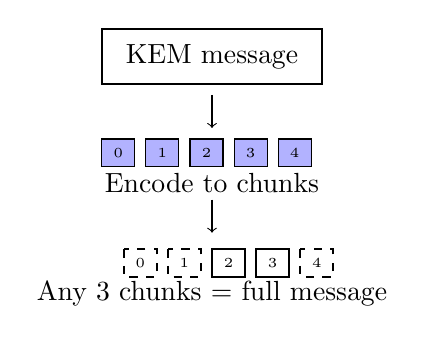
\begin{tikzpicture}[scale=0.7]
					\draw[thick] (0,0) rectangle (4,1) node[midway] {KEM message};
					\draw[->] (2,-0.2) -- (2,-0.8);
					\foreach \x in {0,...,4} {
							\draw[fill=blue!30] (\x*0.8,-1) rectangle (\x*0.8+0.6,-1.5) node[midway,font=\tiny] {\x};
						}
					\node at (2,-1.8) {Encode to chunks};
					\draw[->] (2,-2.1) -- (2,-2.7);
					\draw[thick,dashed] (0.4,-3) rectangle (1,-3.5) node[midway,font=\tiny] {0};
					\draw[thick,dashed] (1.2,-3) rectangle (1.8,-3.5) node[midway,font=\tiny] {1};
					\draw[thick] (2,-3) rectangle (2.6,-3.5) node[midway,font=\tiny] {2};
					\draw[thick] (2.8,-3) rectangle (3.4,-3.5) node[midway,font=\tiny] {3};
					\draw[thick,dashed] (3.6,-3) rectangle (4.2,-3.5) node[midway,font=\tiny] {4};
					\node at (2,-3.8) {Any 3 chunks = full message};
				\end{tikzpicture}
			\end{center}
		\end{column}
	\end{columns}
\end{frame}

\begin{frame}{Katana: Optimized lattice RKEM}{Note: Not yet adopted in Signal}
	\begin{itemize}
		\item \textbf{Ratcheting KEM (RKEM)}: KEM where ciphertext also serves as next public key
		      \begin{itemize}
			      \item Like how Signal reuses $g^b$ for both encryption and next public key
			      \item Saves bandwidth by dual-purposing values
		      \end{itemize}
		\item \textbf{Previous attempts had security flaws}:
		      \begin{itemize}
			      \item Direct lattice translations of Signal's approach were broken
			      \item Required careful fix using hint-MLWE assumption
		      \end{itemize}
		\item \textbf{Katana}: New RKEM based on Kyber
		      \begin{itemize}
			      \item 37\% smaller than naive Kyber approach
			      \item At 192-bit security: 1,416 bytes vs 2,272 bytes
			      \item Provably secure under hint-MLWE
		      \end{itemize}
	\end{itemize}
\end{frame}

\begin{frame}{Triple Ratchet efficiency gains}
	\begin{center}
		\begin{tabular}{|l|c|c|c|}
			\hline
			\textbf{Protocol} & \textbf{Balanced}                   & \textbf{Typing}                     & \textbf{Offline}                     \\
			                  & \textbf{(p=0)}                      & \textbf{(p=0.5)}                    & \textbf{(p=0.9)}                     \\
			\hline
			PQ3               & 6,488 B                             & 11,176 B                            & \textcolor{red}{48,680 B}            \\
			TR + Kyber        & 9,000 B                             & 9,540 B                             & 13,860 B                             \\
			TR + Katana       & \textcolor{green!70!black}{6,500 B} & \textcolor{green!70!black}{6,890 B} & \textcolor{green!70!black}{10,010 B} \\
			\hline
		\end{tabular}
	\end{center}
	\vspace{3mm}
	\begin{itemize}
		\item \textbf{p}: Probability sender continues without waiting for response
		\item \textbf{Balanced}: TR competitive even in best case for PQ3
		\item \textbf{Realistic scenarios}: TR dramatically better (up to 5\times\ improvement)
		\item \textbf{Combines}: Erasure coding + efficient Katana RKEM
	\end{itemize}
\end{frame}

\begin{frame}{Triple Ratchet: Technical challenges}
	\begin{itemize}
		\item \textbf{Desynchronized ratchets}:
		      \begin{itemize}
			      \item Classical and PQ ratchets advance at different speeds
			      \item Need separate root keys for each
			      \item Carefully combine for final message key
		      \end{itemize}
		\item \textbf{Delayed key usage}:
		      \begin{itemize}
			      \item Can't use new PQ key immediately
			      \item Must wait for recipient to decode enough chunks
			      \item Protocol tracks acknowledgments carefully
		      \end{itemize}
		\item \textbf{Security analysis}:
		      \begin{itemize}
			      \item Different epoch functions for classical vs PQ
			      \item PQ healing takes 3 epochs (vs 2 for classical)
			      \item But still provides hybrid security guarantees
		      \end{itemize}
	\end{itemize}
\end{frame}

\begin{frame}{Comparison: PQ3 vs Triple Ratchet}
	\begin{columns}[c]
		\begin{column}{0.5\textwidth}
			\textbf{Apple PQ3:}
			\begin{itemize}
				\item Simple amortization strategy
				\item Full KEM every \approx50 messages
				\item Good for balanced chats
				\item \textcolor{red}{Bad for unbalanced scenarios}
				\item Already deployed
			\end{itemize}
		\end{column}
		\begin{column}{0.5\textwidth}
			\textbf{Signal Triple Ratchet:}
			\begin{itemize}
				\item Sophisticated erasure coding
				\item Chunks spread across messages
				\item Efficient in all scenarios
				\item More complex implementation
				\item Under evaluation
			\end{itemize}
		\end{column}
	\end{columns}
	\vspace{5mm}
	\begin{center}
		\textbf{Key insight}: Different trade-offs for different use cases\\
		Both are significant advances in PQ messaging!
	\end{center}
\end{frame}

\section{Google's Threat Model for Post-Quantum Cryptography}

\begin{frame}{Google as a PQ case study}
	\begin{columns}[c]
		\begin{column}{1\textwidth}
			\begin{itemize}
				\item \textbf{Why look at Google?}
				      \begin{itemize}
					      \item Major cloud provider with diverse crypto needs
					      \item Building their own quantum computer (Google Quantum AI)
					      \item Public about their PQ migration strategy
				      \end{itemize}
				\item \textbf{Google's approach}: Risk-based prioritization
				      \begin{itemize}
					      \item Not all crypto needs equal urgency
					      \item Different algorithms for different use cases
					      \item Timeline-driven deployment
				      \end{itemize}
				\item Let's examine their threat model from 2024\ldots\footnote{\url{https://bughunters.google.com/blog/5108747984306176/google-s-threat-model-for-post-quantum-cryptography}}
			\end{itemize}
		\end{column}
	\end{columns}
\end{frame}

\begin{frame}{Google's prioritization framework}
	\textbf{Four key considerations for quantum threats:}
	\begin{enumerate}
		\item \textbf{Attack feasibility}: How realistic is the quantum attack?
		\item \textbf{Store-now-decrypt-later}: Is data at risk today?
		\item \textbf{Key lifetime}: Do public keys last for decades?
		\item \textbf{Redesign needs}: Will systems need major changes?
	\end{enumerate}
	\vspace{5mm}
	\begin{center}
		\textbf{Not all cryptography is equally threatened}
	\end{center}
\end{frame}

\begin{frame}{Google's crypto taxonomy}
	\begin{columns}[c]
		\begin{column}{0.7\textwidth}
			\textbf{By quantum vulnerability:}
			\begin{enumerate}
				\item \textbf{Asymmetric encryption/KEM}
				      \begin{itemize}
					      \item Broken by Shor's algorithm
					      \item \textcolor{red}{Vulnerable to SNDL (Store-Now-Decrypt-Later)}
				      \end{itemize}
				\item \textbf{Digital signatures}
				      \begin{itemize}
					      \item Broken by Shor's algorithm
					      \item \textcolor{green!70!black}{Not vulnerable to SNDL (Store Now, Decrypt Later)}
				      \end{itemize}
				\item \textbf{``Fancy'' crypto}
				      \begin{itemize}
					      \item Blind signatures, OPRF, etc.
					      \item Case-by-case assessment needed
				      \end{itemize}
				\item \textbf{Symmetric crypto}
				      \begin{itemize}
					      \item \textcolor{green!70!black}{Practically safe from QC}
					      \item Grover's gives only $\sqrt{n}$ speedup
				      \end{itemize}
			\end{enumerate}
		\end{column}
		\begin{column}{0.3\textwidth}
			\begin{center}
				\textbf{Urgency Level}\\[3mm]
				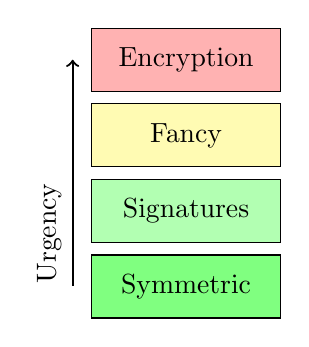
\begin{tikzpicture}[scale=0.8]
					\draw[fill=red!30] (0,0) rectangle (3,1) node[midway] {Encryption};
					\draw[fill=yellow!30] (0,-1.2) rectangle (3,-0.2) node[midway] {Fancy};
					\draw[fill=green!30] (0,-2.4) rectangle (3,-1.4) node[midway] {Signatures};
					\draw[fill=green!50] (0,-3.6) rectangle (3,-2.6) node[midway] {Symmetric};
					\draw[<-,thick] (-0.3,0.5) -- (-0.3,-3.1) node[midway,left=3mm,rotate=90] {Urgency};
				\end{tikzpicture}
			\end{center}
		\end{column}
	\end{columns}
\end{frame}

\begin{frame}{Google's use case analysis}
	\begin{center}
		\begin{tabular}{|l|c|c|c|}
			\hline
			\textbf{Use Case}      & \textbf{SNDL Risk}              & \textbf{Urgency}                & \textbf{Challenge}   \\
			\hline
			\hline
			Encryption in Transit  & \textcolor{red}{High}           & \textcolor{red}{Critical}       & Deployment scale     \\
			(TLS, SSH\ldots)       &                                 &                                 &                      \\
			\hline
			Firmware Signatures    & \textcolor{orange}{Medium}      & \textcolor{red}{High}           & Can't update keys    \\
			(Secure boot)          &                                 &                                 &                      \\
			\hline
			Software Signatures    & \textcolor{green!70!black}{Low} & \textcolor{orange}{Medium}      & Size flexibility     \\
			\hline
			PKI/Certificates       & \textcolor{green!70!black}{Low} & \textcolor{orange}{Medium}      & Chain size explosion \\
			\hline
			Stateless Tokens (JWT) & \textcolor{green!70!black}{Low} & \textcolor{green!70!black}{Low} & 4KB cookie limit     \\
			\hline
		\end{tabular}
	\end{center}
	\vspace{3mm}
	\textbf{Key insight}: Different problems need different solutions
\end{frame}

\begin{frame}{Google's algorithm choices}
	\textbf{Not one-size-fits-all approach:}
	\begin{itemize}
		\item \textbf{Encryption in transit}: ML-KEM-768 + X25519/P256
		      \begin{itemize}
			      \item Most urgent due to SNDL
			      \item Ephemeral keys make deployment easier
		      \end{itemize}
		\item \textbf{Firmware signatures}: SLH-DSA (SPHINCS+)
		      \begin{itemize}
			      \item Can't change keys once burned to silicon
			      \item Hash-based = most conservative choice
			      \item Size less critical than security
		      \end{itemize}
		\item \textbf{Software signatures}: ML-DSA (Dilithium) + classical
		      \begin{itemize}
			      \item Can update keys if needed
			      \item Signing large binaries = performance matters
		      \end{itemize}
	\end{itemize}
\end{frame}

\begin{frame}{The PKI size explosion problem}
	\begin{columns}[c]
		\begin{column}{0.5\textwidth}
			\textbf{Certificate chains today:}
			\begin{itemize}
				\item Root CA: \approx1KB
				\item Intermediate: \approx1KB
				\item Leaf cert: \approx1KB
				\item \textbf{Total}: \approx3KB
			\end{itemize}
			\vspace{5mm}
			\textbf{With PQ signatures:}
			\begin{itemize}
				\item Each cert: >5KB
				\item 3-cert chain: >15KB
				\item \textbf{5\times\ increase!}
			\end{itemize}
		\end{column}
		\begin{column}{0.5\textwidth}
			\textbf{Why this matters:}
			\begin{itemize}
				\item Some devices fail at 10-30KB packets
				\item TLS handshake performance hit
				\item Mobile data costs
			\end{itemize}
			\vspace{5mm}
			\textbf{Google's view:}
			\begin{quote}
				``This problem might be fixable, but a severe performance penalty remains''
			\end{quote}
		\end{column}
	\end{columns}
\end{frame}

\begin{frame}{Timeline: when will quantum computing arrive?}
	\bigimagewithcaption{quantum-threat.png}{Source: Michele Mosca and Marco Piani, Quantum Threat Timeline Report, Global Risk Institute, 2024.}
\end{frame}

\begin{frame}{Timeline: according to Sam Jaques}
	\bigimagewithcaption{quantum-timeline.png}{Source: Sam Jaques}
\end{frame}

\begin{frame}{Threat actors: Who gets QC first?}
	\begin{columns}[c]
		\begin{column}{0.55\textwidth}
			\textbf{1. Nation states}
			\begin{itemize}
				\item Most likely first adopters
				\item Will use ``deniably'' to hide capability
				\item Target: High-value stored data
				\item Focus on static keys (PKI)
			\end{itemize}
			\textbf{2. Insider threats}
			\begin{itemize}
				\item Google builds quantum computers
				\item Crown jewel protection critical
			\end{itemize}
		\end{column}
		\begin{column}{0.45\textwidth}
			\textbf{3. Financially motivated}
			\begin{itemize}
				\item Only when QC becomes cheap
				\item Target: Unmigrated systems
				\item Ransomware potential
			\end{itemize}
			\vspace{5mm}
			\textbf{Key insight}: Different actors = different timelines
		\end{column}
	\end{columns}
\end{frame}

\begin{frame}{Regulatory pressure}
	\begin{itemize}
		\item \textbf{US Government}:
		      \begin{itemize}
			      \item Executive orders requiring PQ migration
			      \item CNSA 2.0: Aggressive timelines for government systems
			      \item FIPS standards coming soon
		      \end{itemize}
		\item \textbf{Europe}:
		      \begin{itemize}
			      \item BSI (Germany) and ANSSI (France) active
			      \item Requesting PQ roadmaps from vendors
		      \end{itemize}
		\item \textbf{Impact on Google}:
		      \begin{itemize}
			      \item Government contracts require compliance
			      \item Accelerates migration timeline
			      \item Can't wait for perfect solutions
		      \end{itemize}
	\end{itemize}
\end{frame}

\begin{frame}{Google's lessons for the industry}
	\begin{enumerate}
		\item \textbf{Prioritize by risk, not uniformly}
		      \begin{itemize}
			      \item Encryption in transit: Do it now
			      \item Signatures: You have more time
		      \end{itemize}
		\item \textbf{Match algorithms to use cases}
		      \begin{itemize}
			      \item No universal ``best'' PQ algorithm
			      \item Consider size, speed, and security trade-offs
		      \end{itemize}
		\item \textbf{Hybrid everything}
		      \begin{itemize}
			      \item PQ algorithms less mature than classical
			      \item Defense against both classical and quantum attacks
		      \end{itemize}
		\item \textbf{Start experimenting now}
		      \begin{itemize}
			      \item PKI and tokens need creative solutions
			      \item Industry collaboration essential
		      \end{itemize}
	\end{enumerate}
\end{frame}

\section{How Things Can Go Wrong}

\begin{frame}{Reality check: Post-quantum isn't perfect}
	\begin{itemize}
		\item \textbf{Post-quantum $\neq$ unbreakable}
		\item \textbf{Fundamental challenge}: These schemes are newer
		      \begin{itemize}
			      \item RSA: 40+ years of cryptanalysis
			      \item Elliptic curves: 30+ years
			      \item Most PQ schemes: 10-20 years
		      \end{itemize}
		\item \textbf{Limited understanding brings risks}:
		      \begin{itemize}
			      \item Security levels harder to quantify
			      \item Implementation pitfalls less understood
			      \item Potential for unexpected attacks
		      \end{itemize}
		\item Let's explore what can go wrong\ldots
	\end{itemize}
\end{frame}

\subsection{Unclear Security Levels}

\begin{frame}{The deceptive strength problem}
	\begin{columns}[c]
		\begin{column}{1\textwidth}
			\begin{itemize}
				\item \textbf{Some schemes look incredibly strong on paper\ldots}
				\item \textbf{Example}: McEliece (hardness of decoding a linear code with insufficient information)
				      \begin{itemize}
					      \item In the worst case, some argue could be proven NP-hard
					      \item Sounds amazing: NP-hard = practically unbreakable!
					      \item But cryptographic problems are based on the average case, not the worst case\ldots
					      \item And the claim of NP-hardness even here is debated\ldots\footnote{Eurocrypt 2025 paper found a subexponential distinguisher for McEliece: \url{https://appliedcryptography.page/paper/\#syzygy-distinguisher}}
				      \end{itemize}
				\item \textbf{Real-world complications}:
				      \begin{itemize}
					      \item Security proofs only work for certain parameters
					      \item Practical implementations use different parameters
					      \item The gap between theory and practice can be exploited
				      \end{itemize}
			\end{itemize}
		\end{column}
	\end{columns}
\end{frame}

\begin{frame}{Asymptotic vs. concrete security}
	\begin{columns}[c]
		\begin{column}{0.5\textwidth}
			\textbf{Asymptotic security:}
			\begin{itemize}
				\item ``Secure as $n \rightarrow \infty$''
				\item Mathematical proofs assume large parameters
				\item Example: ``Secure for lattice dimension $> 10^6$''
			\end{itemize}
			\textbf{Concrete security:}
			\begin{itemize}
				\item What we actually use: $n = 512$
				\item May be far from asymptotic regime
				\item Security at practical parameters unclear
			\end{itemize}
		\end{column}
		\begin{column}{0.5\textwidth}
			\begin{center}
				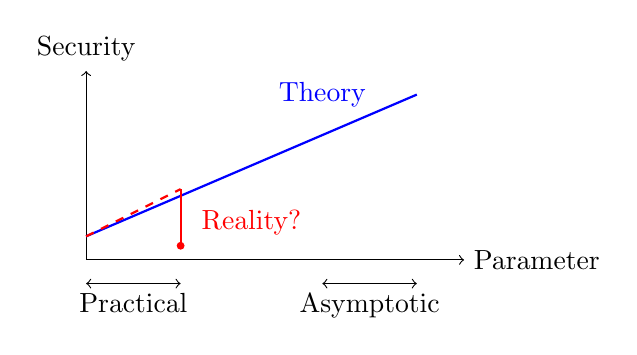
\begin{tikzpicture}[scale=0.6]
					\draw[->] (0,0) -- (8,0) node[right] {Parameter};
					\draw[->] (0,0) -- (0,4) node[above] {Security};
					\draw[thick,blue] (0,0.5) -- (7,3.5);
					\draw[thick,red,dashed] (0,0.5) -- (2,1.5);
					\draw[thick,red] (2,1.5) -- (2,0.3);
					\filldraw[red] (2,0.3) circle (2pt);
					\draw[<->] (0,-0.5) -- (2,-0.5) node[midway,below] {Practical};
					\draw[<->] (5,-0.5) -- (7,-0.5) node[midway,below] {Asymptotic};
					\node[blue] at (5,3.5) {Theory};
					\node[red] at (3.5,0.8) {Reality?};
				\end{tikzpicture}
			\end{center}
		\end{column}
	\end{columns}
\end{frame}

\begin{frame}{The unknown attack landscape}
	\begin{itemize}
		\item \textbf{With RSA}: We know strong attacks
		      \begin{itemize}
			      \item Number Field Sieve for factoring
			      \item Decades of optimization
			      \item Can estimate security precisely
		      \end{itemize}
		\item \textbf{With lattice-based crypto}: Still discovering attacks
		      \begin{itemize}
			      \item New attack improvements regularly published
			      \item Hard to predict future improvements
			      \item Security estimates keep changing
		      \end{itemize}
		\item \textbf{Example}: NIST Round 2 eliminations
		      \begin{itemize}
			      \item Several ``secure'' schemes broken during competition
			      \item Some had security proofs!
			      \item Proofs were correct, but assumptions weren't
		      \end{itemize}
	\end{itemize}
\end{frame}

\subsection{When Quantum Computers Arrive}
\begin{frame}{Breaking news from 2052\ldots}
	\begin{itemize}
		\item \textbf{The nightmare scenario}: Large quantum computer suddenly exists
		\item \textbf{All classical crypto broken overnight}
		\item \textbf{Common misconception}: ``Signatures are recoverable, encryption isn't''
		\item \textbf{Reality}: It depends on where the crypto lives\ldots
	\end{itemize}
\end{frame}

\begin{frame}{Digital signatures: Not always recoverable}
	\begin{columns}[c]
		\begin{column}{0.5\textwidth}
			\textbf{Software signatures:}
			\begin{itemize}
				\item Generate new PQ keys
				\item Re-sign and re-deploy
				\item Revoke old keys
				\item \textcolor{green!70!black}{Recoverable}
			\end{itemize}
			\vspace{3mm}
			\textbf{Hardware signatures:}
			\begin{itemize}
				\item Keys burned in ROM/fuses
				\item Can't update silicon
				\item Foundation of all security
				\item \textcolor{red}{Permanently broken}
			\end{itemize}
		\end{column}
		\begin{column}{0.5\textwidth}
			\begin{center}
				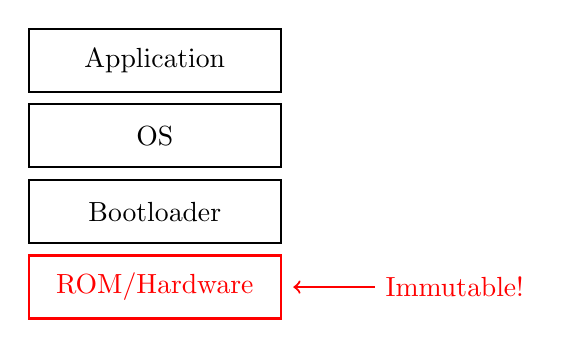
\begin{tikzpicture}[scale=0.8]
					\draw[thick] (0,0) rectangle (4,1) node[midway] {Application};
					\draw[thick] (0,-1.2) rectangle (4,-0.2) node[midway] {OS};
					\draw[thick] (0,-2.4) rectangle (4,-1.4) node[midway] {Bootloader};
					\draw[thick,red] (0,-3.6) rectangle (4,-2.6) node[midway] {ROM/Hardware};
					\draw[<-,red,thick] (4.2,-3.1) -- (5.5,-3.1) node[right] {Immutable!};
				\end{tikzpicture}
			\end{center}
		\end{column}
	\end{columns}
\end{frame}

\begin{frame}{The hardware root of trust problem}
	\begin{itemize}
		\item \textbf{Every device starts with hardware-based security:}
		      \begin{itemize}
			      \item ROM code executes first
			      \item Public keys in fuses/OTP memory
			      \item Hardware crypto accelerators
			      \item Debug unlock mechanisms
		      \end{itemize}
		\item \textbf{Secure boot chain}: Each stage verifies the next
		      \begin{itemize}
			      \item ROM verifies bootloader signature
			      \item Bootloader verifies OS signature
			      \item OS verifies application signatures
		      \end{itemize}
		\item \textbf{If ROM keys are broken}: \textcolor{red}{Entire chain collapses}
		      \begin{itemize}
			      \item Can install any bootloader
			      \item Bypass all security checks
			      \item Device permanently compromised
		      \end{itemize}
	\end{itemize}
\end{frame}

\begin{frame}{Long-lived infrastructure: The real disaster}
	\begin{columns}[c]
		\begin{column}{0.55\textwidth}
			\textbf{Consumer devices:}
			\begin{itemize}
				\item Phones: 2-3 year lifecycle
				\item Laptops: 3-5 years
				\item \textcolor{green!70!black}{Painful but manageable}
			\end{itemize}
			\vspace{3mm}
			\textbf{Critical infrastructure:}
			\begin{itemize}
				\item Power plants: 30-50 years?
				\item Aircraft: 20-30 years?
				\item Satellites: 10-15 years?
				\item Military systems: 20-40 years?
				\item \textcolor{red}{Replacement = \$billions}
			\end{itemize}
		\end{column}
		\begin{column}{0.45\textwidth}
			\textbf{The \$20 chip problem:}
			\begin{itemize}
				\item Cheap secure element
				\item Deeply embedded everywhere
				\item Controls \$1M+ equipment
				\item Can't extract and replace
			\end{itemize}
			\vspace{3mm}
			\textbf{Example}: Car ECUs
			\begin{itemize}
				\item Cars may have multiple ECUs
				\item Each has secure boot
				\item Cars last 10-20 years
			\end{itemize}
		\end{column}
	\end{columns}
\end{frame}

\begin{frame}{Encryption vs signatures: Both can be catastrophic}
	\begin{center}
		\begin{tabular}{|l|c|c|}
			\hline
			\textbf{Attack Type}     & \textbf{Encryption}      & \textbf{Signatures}        \\
			\hline
			\hline
			\textbf{Past data}       & \textcolor{red}{Exposed} & Historical record damaged  \\
			\hline
			\textbf{Future security} & Can use PQ crypto        & \textcolor{red}{HW broken} \\
			\hline
			\textbf{Recovery cost}   & Re-encrypt (if possible) & Replace hardware           \\
			\hline
			\textbf{Timeline}        & Immediate exposure       & Permanent vulnerability    \\
			\hline
			\textbf{Worst case}      & Secrets revealed         & Infrastructure compromised \\
			\hline
		\end{tabular}
	\end{center}
	\vspace{3mm}
	\begin{center}
		\textbf{Reality}: Both are potential disasters with different characteristics
	\end{center}
\end{frame}

\begin{frame}{Real-world impact of broken hardware signatures}
	\begin{itemize}
		\item \textbf{Secure boot bypass}: Install any firmware
		      \begin{itemize}
			      \item Persistent malware
			      \item Undetectable rootkits
			      \item Complete device control
		      \end{itemize}
		\item \textbf{Debug interface unlock}: Full hardware access
		      \begin{itemize}
			      \item Extract all secrets
			      \item Modify hardware behavior
			      \item Bypass all protections
		      \end{itemize}
		\item \textbf{Supply chain attacks}: Counterfeit components
		      \begin{itemize}
			      \item Fake firmware updates
			      \item Trojan hardware accepted as genuine
			      \item No way to verify authenticity
		      \end{itemize}
	\end{itemize}
\end{frame}

\begin{frame}{The true cost of ``Q-day'' for signatures}
	\begin{columns}[c]
		\begin{column}{0.5\textwidth}
			\textbf{Software systems:}
			\begin{itemize}
				\item Cost: Engineering time
				\item Timeline: Weeks to months
				\item Impact: Service disruption
			\end{itemize}
			\vspace{5mm}
			\textbf{Hardware systems:}
			\begin{itemize}
				\item Cost: Full replacement
				\item Timeline: Years to decades
				\item Impact: Systemic failure
			\end{itemize}
		\end{column}
		\begin{column}{0.5\textwidth}
			\textbf{Cost estimates:}
			\begin{itemize}
				\item Power grid: Billions?
				\item Military fleet: Billions?
				\item Global auto industry: Trillions?
				\item Satellite constellation: Who knows
			\end{itemize}
			\vspace{3mm}
			\textbf{Bottom line}: Potentially massive cost
		\end{column}
	\end{columns}
\end{frame}

\begin{frame}{Key agreement: It's complicated}
	\begin{columns}[c]
		\begin{column}{1\textwidth}
			\textbf{Simple Diffie-Hellman:}
			\begin{itemize}
				\item Alice: $g^a$, Bob: $g^b$
				\item Shared: $g^{ab}$
				\item \textcolor{red}{Quantum computer recovers $a$ or $b$}
				\item \textcolor{red}{All past communications compromised}
			\end{itemize}

			\textbf{Modern protocols (Signal):}
			\begin{itemize}
				\item New DH for each message
				\item Keys depend on message history
				\item Even with QC, need full conversation
				\item \textcolor{green!70!black}{Much harder to break retroactively}
			\end{itemize}
		\end{column}
	\end{columns}
\end{frame}

\subsection{Implementation Vulnerabilities}

\begin{frame}{The implementation gap}
	\begin{center}
		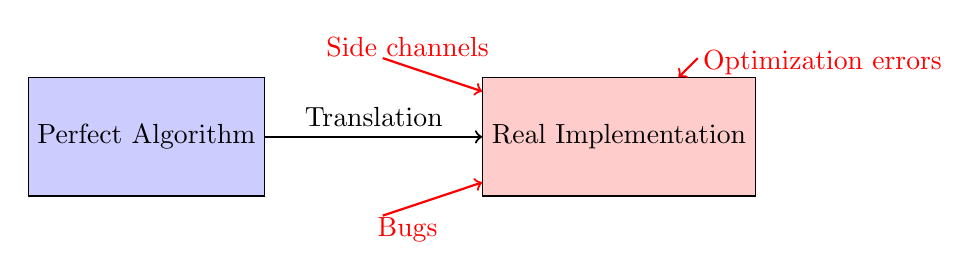
\begin{tikzpicture}[scale=1]
			\node[draw,rectangle,minimum width=3cm,minimum height=1.5cm,fill=blue!20] (theory) at (0,0) {Perfect Algorithm};
			\node[draw,rectangle,minimum width=3cm,minimum height=1.5cm,fill=red!20] (practice) at (6,0) {Real Implementation};
			\draw[->,thick] (theory) -- (practice) node[midway,above] {Translation};
			\draw[->,thick,red] (3,-1) -- (practice) node[near start,below] {Bugs};
			\draw[->,thick,red] (3,1) -- (practice) node[near start,above] {Side channels};
			\draw[->,thick,red] (7,1) -- (practice) node[near start,right] {Optimization errors};
		\end{tikzpicture}
	\end{center}
	\begin{itemize}
		\item \textbf{Theory}: Algorithm is perfectly secure
		\item \textbf{Practice}: Implementation has vulnerabilities
		\item \textbf{The gap}: Where security breaks down
	\end{itemize}
\end{frame}

\begin{frame}[fragile]{A cautionary tale: The semicolon bug}
	\begin{columns}[c]
		\begin{column}{0.6\textwidth}
			\textbf{Actual bug in Apple's SSL/TLS (2014):}
			\begin{verbatim}
if ((err = SSLHashSHA1.update(&hashCtx,
      &signedParams)) != 0)
    goto fail;
    goto fail;  // <-- Extra goto!
// This code always skipped:
if ((err = SSLHashSHA1.final(&hashCtx,
      &hashOut)) != 0)
    goto fail;
   \end{verbatim}
		\end{column}
		\begin{column}{0.4\textwidth}
			\textbf{Impact:}
			\begin{itemize}
				\item Signature verification bypassed
				\item Any certificate accepted
				\item Complete security failure
				\item From one duplicated line!
			\end{itemize}

			\textbf{Lesson:} Even ``unbreakable'' crypto fails with implementation bugs
		\end{column}
	\end{columns}
\end{frame}

\begin{frame}{Side-channel attacks: The hidden threat}
	\begin{itemize}
		\item \textbf{What are side channels?}
		      \begin{itemize}
			      \item Information leaked during computation
			      \item Not through the algorithm itself
			      \item Through physical effects
		      \end{itemize}
		\item \textbf{Common side channels}:
		      \begin{itemize}
			      \item \textbf{Timing}: Operations take different times
			      \item \textbf{Power}: Different operations use different power
			      \item \textbf{Cache}: Memory access patterns reveal secrets
			      \item \textbf{Electromagnetic}: EM emissions during computation
		      \end{itemize}
		\item \textbf{Why PQ crypto is vulnerable}: Complex mathematical operations
		      \begin{itemize}
			      \item Matrix multiplications (lattice-based)
			      \item Polynomial operations (code-based)
			      \item Many conditional branches
		      \end{itemize}
	\end{itemize}
\end{frame}

\begin{frame}{KyberSlash: A real-world PQ vulnerability}
	\begin{columns}[c]
		\begin{column}{1\textwidth}
			\begin{itemize}
				\item \textbf{What}: Timing attack on Kyber implementations\footnote{\url{https://appliedcryptography.page/paper/\#kyber-slash}} (Dec 2023)
				\item \textbf{Affected}: Multiple ``production-ready'' Kyber libraries
				\item \textbf{The vulnerability}:
				      \begin{itemize}
					      \item Division operations in decoding took variable time
					      \item Time depended on secret polynomial coefficients
					      \item Attacker measures decryption times
					      \item Recovers secret key within a couple million queries
				      \end{itemize}
				\item \textbf{Impact}: Complete key recovery in ``secure'' implementations!
				\item \textbf{Lesson}: Even NIST-standardized PQ crypto had critical flaws
				      \begin{itemize}
					      \item Years of review missed this
					      \item ``Constant-time'' code wasn't
					      \item Shows immaturity of PQ implementations
				      \end{itemize}
			\end{itemize}
		\end{column}
	\end{columns}
\end{frame}

\begin{frame}{Timing attacks on post-quantum cryptography}
	\begin{columns}[c]
		\begin{column}{0.5\textwidth}
			\textbf{Example: Gaussian sampling in lattices}
			\begin{itemize}
				\item Need to sample from discrete Gaussian
				\item Rejection sampling: variable time
				\item Time depends on secret values!
			\end{itemize}

			\textbf{Attack scenario:}
			\begin{enumerate}
				\item Measure decryption times
				\item Infer error vector properties
				\item Recover secret key
			\end{enumerate}
		\end{column}
		\begin{column}{0.5\textwidth}
			\begin{center}
				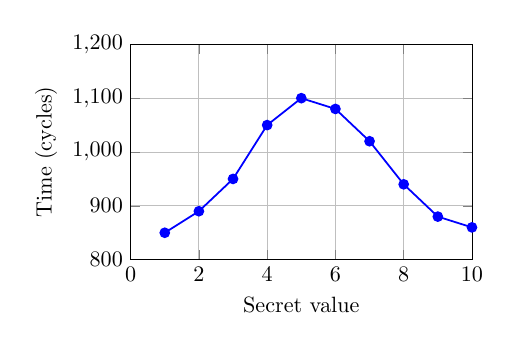
\begin{tikzpicture}[scale=0.8]
					\begin{axis}[
							xlabel={Secret value},
							ylabel={Time (cycles)},
							xmin=0, xmax=10,
							ymin=800, ymax=1200,
							width=7cm,
							height=5cm,
							grid=major,
						]
						\addplot[blue, thick, mark=*, mark size=2pt] coordinates {
								(1,850) (2,890) (3,950) (4,1050)
								(5,1100) (6,1080) (7,1020) (8,940)
								(9,880) (10,860)
							};
					\end{axis}
				\end{tikzpicture}

				Timing reveals secret information!
			\end{center}
		\end{column}
	\end{columns}
\end{frame}

\begin{frame}{The PQ paradox}
	\begin{itemize}
		\item PQ schemes may initially be LESS secure than classical!
		\item \textbf{Why?}
		      \begin{itemize}
			      \item RSA/ECC: 40 years of implementation hardening
			      \item Constant-time implementations well understood
			      \item Side-channel protections mature
		      \end{itemize}
		\item \textbf{Post-quantum crypto}:
		      \begin{itemize}
			      \item New implementations = new bugs
			      \item Complex operations = more side channels
			      \item Less implementation experience
		      \end{itemize}
		\item \textbf{Timeline of maturity}:
		      \begin{itemize}
			      \item Years 1-5: Discovering vulnerabilities
			      \item Years 5-10: Developing countermeasures
			      \item Years 10+: Mature, hardened implementations
		      \end{itemize}
	\end{itemize}
\end{frame}

\begin{frame}{Lessons learned}
	\begin{itemize}
		\item \textbf{Post-quantum $\neq$ post-security-concerns}
		\item \textbf{Key challenges remain}:
		      \begin{enumerate}
			      \item Unclear concrete security levels
			      \item Implementation vulnerabilities
			      \item Side-channel attacks
			      \item The ``store now, decrypt later'' threat
		      \end{enumerate}
		\item \textbf{Best practices}:
		      \begin{itemize}
			      \item Use conservative parameters
			      \item Implement hybrid solutions (classical + PQ)
			      \item Invest in secure implementations
			      \item Plan for crypto-agility
		      \end{itemize}
	\end{itemize}
\end{frame}

\begin{frame}[plain]
	\titlepage
\end{frame}
\end{document}
